% =============================================================
%  Three-level Vienna rectifier on the 690 V grid: the model vienna_rectifier
%  pwr-control documentation - compile with pdflatex (three times) from inside this folder:
%      pdflatex vienna_rectifier.tex  (x3)
%  Block diagrams and the circuit of the leg are drawn in this file (TikZ, circuitikz). The figures of
%  figures/*.pdf and every number of the note come from the companion scripts of py/ (numpy, scipy, numba,
%  matplotlib):
%      cd py && python3 vienna_design_check.py ../figures   -> ../figures/*.pdf, vienna_design_check_output.txt
%  vienna_design_check.py repeats the linear checks of private/vienna_design.m of the model and runs the switched
%  replica of the model, py/vienna_sim.py.
% =============================================================
\documentclass[11pt,a4paper]{scrartcl}
% ===================== PACKAGES =====================
\usepackage[british]{babel}
\usepackage[tmargin=1in, bmargin=1in, lmargin=0.75in, rmargin=0.75in]{geometry}
\usepackage[dvipsnames,table]{xcolor}  % prima di tikz, listings, ecc.

\usepackage{tikz}
\usepackage{graphicx}
\usepackage{pgfplots}
\pgfplotsset{width=12cm, compat=1.9}
\usepackage{setspace}
\usepackage{chemmacros}
\usepackage{chemfig}
\usepackage{esint}
\usepackage{tabularray}
\usepackage{makeidx}
\usepackage{epstopdf}
\usepackage{amssymb}
\usepackage{mathrsfs}
\usepackage{bm}
\usepackage{amsmath}
\usepackage{enumitem}
\usepackage[english]{varioref}
\usepackage{lipsum}
\usepackage{fancyhdr}
\usepackage{float}
\usepackage{empheq}
\usepackage[framemethod=tikz]{mdframed}
\numberwithin{equation}{section}
\usepackage{eso-pic}
\usepackage{calc}
\usepackage{nccmath}
\usepackage{caption}
\usepackage{subcaption}
\usepackage{gensymb}
\usepackage{amsfonts, amsthm, epsfig, epstopdf, titling, url, array}
\usepackage{tabularx}
\usepackage{makecell}
\usepackage{booktabs}
\usepackage{array}
\usepackage{siunitx}
\sisetup{input-digits=0123456789\pi}
\usepackage[symbol]{footmisc}
\usepackage{multicol}
\usepackage{boondox-cal}
\usepackage{blindtext}
\usepackage{changepage}
\usepackage{nomencl}
\usepackage{hyperref}
\usepackage{xurl}
\usepackage{ragged2e}
\usepackage[version=4]{mhchem}  % ← conflitto di opzioni
\usepackage{longtable}
\usepackage{chemformula}
\usetikzlibrary{arrows.meta,positioning,calc}

% ===================== SI UNITS =====================
\DeclareSIUnit\atm{atm}
\DeclareSIUnit{\var}{var}
\DeclareSIUnit{\pu}{p.u.}


% ===================== MATH OPERATORS =====================
\DeclareMathOperator{\rank}{rank}
\DeclareMathOperator{\atantwo}{atan2}
\DeclareMathOperator{\spn}{span}

% ===================== COMMANDS =====================
\newcommand{\abs}[1]{\left|#1\right|}
\newcommand{\sign}{\text{sign}}
\newcommand{\centered}[1]{\begin{tabular}{@{}l@{}} #1 \end{tabular}}

% ===================== COLORS =====================
\definecolor{mycolor1}{rgb}{0.97, 0.97, 0.97}
\definecolor{mycolor2}{rgb}{0.97, 0.97, 0.97}
\definecolor{tableShade}{gray}{0.9}

% ===================== THEOREM ENVIRONMENTS =====================
\theoremstyle{it}
\newtheorem{defn}{Definition}[section]
\newtheorem{assumption}{Assumption}[section]
\newtheorem{thm}{Theorem}[section]
\newtheorem{lemma}{Lemma}[section]
\newtheorem{corollary}{Corollary}[section]
\theoremstyle{definition}
\newtheorem{example}{Example}[section]

% ===================== CUSTOM ENVIRONMENTS =====================
\newenvironment{myitemize_1}{
	\begin{itemize}[topsep=0pt]
		\setlength{\topsep}{2pt}
		\setlength{\itemsep}{2pt}
		\setlength{\parskip}{2pt}
		\setlength{\parsep}{2pt}
	}{\end{itemize}}

\newmdenv[
innerlinewidth=0.5pt,
roundcorner=4pt,
backgroundcolor=mycolor2,
linecolor=mycolor1,
innerleftmargin=6pt,
innerrightmargin=6pt,
innertopmargin=6pt,
innerbottommargin=6pt
]{mybox}

% ===================== TABLE COLUMN TYPES =====================
\newcolumntype{Y}{>{\hsize=2\hsize}X}
\newcolumntype{Z}{>{\centering\arraybackslash\hsize=0.857\hsize}X}

% ===================== SECTION DEPTH =====================
\setcounter{secnumdepth}{3}
\setcounter{tocdepth}{3}

% ===================== PAGE STYLE =====================
\setlength{\headheight}{20pt}
\setlength{\headsep}{20pt}

\pagestyle{fancy}
\fancypagestyle{firstpage}{\rhead{}}
\fancyhead[L]{\slshape\nouppercase{\leftmark}}
\chead{}
\rhead{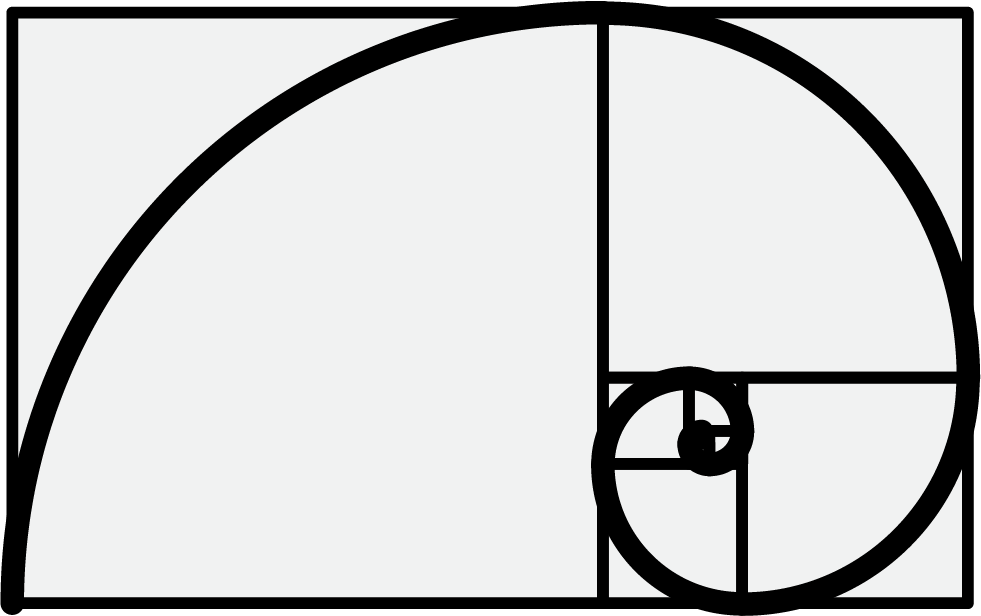
\includegraphics[height=0.75cm]{../../AAA_template_latex_settings/pwr-control_logo_doc.png}}
\lfoot{\href{http://www.pwr-control.com}{pwr-control.com}}
\cfoot{-\ \thepage\ -}
\rfoot{\textit{}}
\renewcommand{\headrulewidth}{0.4pt}
\renewcommand{\footrulewidth}{0.4pt}


\geometry{
	a4paper,
	top    = 2.5cm,
	bottom = 3.0cm,
	left   = 2.5cm,
	right  = 2.5cm
}

\hypersetup{
	colorlinks = true,
	urlcolor   = blue,
	linkcolor  = black,
	citecolor  = black
}

\pagenumbering{gobble}

\usepackage[american]{circuitikz}
\usetikzlibrary{shapes.geometric,fit,calc}

\newcommand{\ped}[1]{_{\mathrm{#1}}}
\newcommand{\code}[1]{\texttt{#1}}
\newcommand{\us}{\_\allowbreak}  % breakable underscore for long paths
\renewcommand{\tabularxcolumn}[1]{>{\raggedright\arraybackslash}p{#1}}
\setlength{\emergencystretch}{3em}
\sisetup{per-mode=symbol,retain-explicit-plus}

% ---------------- document metadata (read by the title page) ----------------
\newcommand{\DocCategory}{Technical Note}
\newcommand{\DocField}{Power Electronics and Control Systems}

\newcommand{\DocTitle}{%
	{\fontsize{20}{24}\selectfont\bfseries Three-level Vienna rectifier\\ on the \SI{690}{\volt} grid\par}
	\vspace{14pt}
	{\fontsize{16}{23}\selectfont\bfseries \code{vienna\_rectifier}: power stage and control,\\ fixes of November 2026, design check of the loops,\\ start-up, steady state and open points\par}
}

\newcommand{\DocSubtitle}{%
	The model \code{vienna\_rectifier} of \code{pwr-control/modelization-and-control} after the revision of November 2026: what it contains, why it did not run, what was changed in the model and in its initialization, how its loops are designed, and how it behaves at the start and in steady state, checked with linear models and with a switched replica of the model.
}

\newcommand{\DocAuthor}{Davide Bagnara}
\newcommand{\DocRevision}{00}
\newcommand{\DocDate}{November 2026}

\newcommand{\DocAbstract}{%
	The model \code{vienna\_rectifier} feeds a \SI{250}{\kilo\watt} three-level Vienna rectifier from a \SI{1}{\mega\volt\ampere}, \SI{690}{\volt} grid emulator through an LCL filter whose grid side is the leakage of the Dyn11 transformer; the split DC link (\num{2} $\times$ \SI{14.4}{\milli\farad}) supplies a \SI{5}{\ohm} load, \SI{229}{\kilo\watt} at \SI{1070}{\volt}. The control is the dq control of the AFE models of the repository: DDSRF-PLL, DC-voltage PI, vector PI of the converter current, space vector modulation and three-level PWM at \SI{4}{\kilo\hertz} with double update. As saved, the model did not run: no initialization gave the \code{param.*} names that the grid emulator read, the current PI read the gains of a PMSM inverter, a bus object and the names of the modulator lines were missing, 23 From blocks had no Goto, and the DDSRF-PLL was fed with the negative sequence and could not lock (\SI{1383}{\ampere} peaks and \SI{1916}{\volt} on the DC link in the switched replica). This note describes the model, the new initialization with the struct \code{param} and the changes to the model, and checks the design: operating point (\num{8.7}~\% of voltage margin), LCL resonance at \SI{1381}{\hertz}, just above $f\ped{s}/6$, current loop (\SI{135}{\hertz}, \ang{70} of phase margin), DC-voltage loop (\SI{21}{\hertz}, \ang{98}), DDSRF-PLL with its decoupling filter in the loop (\ang{58}), neutral-point ripple (\SI{5.4}{\volt} peak to peak). A switched replica of the model gives the start-up (\SI{752}{\ampere} peak, DC link between \SI{758}{} and \SI{1171}{\volt}) and the steady state (THD of the grid current \num{3.4}~\%). The start-up peak comes from the anti-windup of the DC-voltage PI, which drives the current reference positive while the DC voltage is still above its reference, and from the current loop, which has no feed-forward of the grid voltage. Changes quantified but not applied: a DC-voltage PI with lower limit 0 and conditional integration (\SI{456}{\ampere}, no overshoot), or a feed-forward of the capacitor voltage with a DC-voltage reference that starts from the measured voltage (\SI{455}{\ampere}, no overshoot); a zero sequence that follows the sign of the current (THD \num{2.5}~\%).
}

\newcommand{\RevisionHistory}{%
	00 & November 2026 & First issue: model, changes of November 2026, design check, switched replica of the start-up and of the steady state, open points; scripts \code{py/vienna\_sim.py} and \code{py/vienna\_design\_check.py}. & \DocAuthor \\
}

\newcommand{\MetaLabelA}{Project Repository}
\newcommand{\MetaValueAUrl}{https://github.com/pwr-control/modelization-and-control.git}
\newcommand{\MetaValueALabel}{modelization-and-control.git (vienna\_rectifier)}

\newcommand{\MetaLabelB}{Framework}
\newcommand{\MetaValueB}{MATLAB/Simulink, Python}

\begin{document}

% =============================================================
%  pwr-control LaTeX template - FRONTESPIZIO
%
%  Da richiamare come prima istruzione dopo \begin{document}:
%      % =============================================================
%  pwr-control LaTeX template - FRONTESPIZIO
%
%  Da richiamare come prima istruzione dopo \begin{document}:
%      % =============================================================
%  pwr-control LaTeX template - FRONTESPIZIO
%
%  Da richiamare come prima istruzione dopo \begin{document}:
%      \input{../../AAA_template_latex_settings/titlepage}
%
%  Il documento deve definire prima di \begin{document}:
%      \DocCategory   categoria del documento
%      \DocField      area tecnica
%      \DocTitle      titolo (una o due righe)
%      \DocSubtitle   sottotitolo
%      \DocAuthor     autore/i, separati da virgola
%      \DocRevision   numero di revisione corrente (es. 00)
%      \DocDate       data della revisione corrente
%      \DocAbstract   abstract
%      \RevisionHistory  righe della tabella di revisione, nel formato
%                        Rev. & Date & Description & Authors \\
%      \MetaLabelA \MetaValueAUrl \MetaValueALabel
%      \MetaLabelB \MetaValueB
% =============================================================

\providecommand{\DocCategory}{Technical Research Report}
\providecommand{\DocField}{Power Electronics and Control Systems}
\providecommand{\DocSubtitle}{}
\providecommand{\DocRevision}{00}
\providecommand{\DocAbstract}{}
\providecommand{\RevisionHistory}{%
	\DocRevision & \DocDate & First issue. & \DocAuthor \\
}

\titlepage

% ---- Intestazione centrata ----
\begin{center}
	{\Large\scshape \DocCategory}\\[8pt]
	{\large\scshape \DocField}
\end{center}

\vspace{30pt plus 4pt minus 14pt}
\noindent\rule{\linewidth}{0.8pt}

% ---- Titolo ----
\begin{center}
	\DocTitle
\end{center}

\vspace{4pt}
\noindent\rule{\linewidth}{2.2pt}

% ---- Sottotitolo ----
\begin{center}
	\begin{onehalfspace}
		{\large\itshape \DocSubtitle}
	\end{onehalfspace}
\end{center}

% ---- Authors / Revision / Date ----
\vspace{30pt plus 4pt minus 14pt}

\noindent
\begin{minipage}[t]{0.46\linewidth}
	\raggedright
	\textbf{Authors:}\\[2pt]
	\DocAuthor
\end{minipage}%
\hfill
\begin{minipage}[t]{0.22\linewidth}
	\centering
	\textbf{Revision:}\\[2pt]
	\DocRevision
\end{minipage}%
\hfill
\begin{minipage}[t]{0.30\linewidth}
	\raggedleft
	\textbf{Date:}\\[2pt]
	\DocDate
\end{minipage}

\vspace{10pt}
\noindent\rule{\linewidth}{0.8pt}

% ---- Abstract ----
\vspace{24pt plus 4pt minus 12pt}

\begin{center}
	\begin{minipage}{0.88\linewidth}
		\footnotesize
		\begin{onehalfspace}
			\textbf{Abstract:} \DocAbstract
		\end{onehalfspace}
	\end{minipage}
\end{center}

\vfill

% ---- Revision history ----
\begin{center}
	\begin{minipage}{0.96\linewidth}
		\centering
		{\footnotesize\scshape Revision history}\\[6pt]
		{\footnotesize
			\begin{tabular}{@{}cl>{\raggedright\arraybackslash}p{0.36\linewidth}>{\raggedright\arraybackslash}p{0.28\linewidth}@{}}
				\toprule
				\textbf{Rev.} & \textbf{Date} & \textbf{Description} & \textbf{Authors} \\
				\midrule
				\RevisionHistory
				\bottomrule
			\end{tabular}}
	\end{minipage}
\end{center}

\vspace{18pt plus 4pt minus 10pt}

% ---- Metadati in fondo ----
\noindent
\begin{tabular}{@{} r @{\quad} l @{}}
	\textsc{\MetaLabelA:} & {\href{\MetaValueAUrl}{\MetaValueALabel}} \\[3pt]
	\textsc{\MetaLabelB:} & {\MetaValueB}       \\[3pt]
\end{tabular}

% =============================================================
%  Fine frontespizio
% =============================================================
\newpage
\pagenumbering{arabic}
\setcounter{page}{1}

%
%  Il documento deve definire prima di \begin{document}:
%      \DocCategory   categoria del documento
%      \DocField      area tecnica
%      \DocTitle      titolo (una o due righe)
%      \DocSubtitle   sottotitolo
%      \DocAuthor     autore/i, separati da virgola
%      \DocRevision   numero di revisione corrente (es. 00)
%      \DocDate       data della revisione corrente
%      \DocAbstract   abstract
%      \RevisionHistory  righe della tabella di revisione, nel formato
%                        Rev. & Date & Description & Authors \\
%      \MetaLabelA \MetaValueAUrl \MetaValueALabel
%      \MetaLabelB \MetaValueB
% =============================================================

\providecommand{\DocCategory}{Technical Research Report}
\providecommand{\DocField}{Power Electronics and Control Systems}
\providecommand{\DocSubtitle}{}
\providecommand{\DocRevision}{00}
\providecommand{\DocAbstract}{}
\providecommand{\RevisionHistory}{%
	\DocRevision & \DocDate & First issue. & \DocAuthor \\
}

\titlepage

% ---- Intestazione centrata ----
\begin{center}
	{\Large\scshape \DocCategory}\\[8pt]
	{\large\scshape \DocField}
\end{center}

\vspace{30pt plus 4pt minus 14pt}
\noindent\rule{\linewidth}{0.8pt}

% ---- Titolo ----
\begin{center}
	\DocTitle
\end{center}

\vspace{4pt}
\noindent\rule{\linewidth}{2.2pt}

% ---- Sottotitolo ----
\begin{center}
	\begin{onehalfspace}
		{\large\itshape \DocSubtitle}
	\end{onehalfspace}
\end{center}

% ---- Authors / Revision / Date ----
\vspace{30pt plus 4pt minus 14pt}

\noindent
\begin{minipage}[t]{0.46\linewidth}
	\raggedright
	\textbf{Authors:}\\[2pt]
	\DocAuthor
\end{minipage}%
\hfill
\begin{minipage}[t]{0.22\linewidth}
	\centering
	\textbf{Revision:}\\[2pt]
	\DocRevision
\end{minipage}%
\hfill
\begin{minipage}[t]{0.30\linewidth}
	\raggedleft
	\textbf{Date:}\\[2pt]
	\DocDate
\end{minipage}

\vspace{10pt}
\noindent\rule{\linewidth}{0.8pt}

% ---- Abstract ----
\vspace{24pt plus 4pt minus 12pt}

\begin{center}
	\begin{minipage}{0.88\linewidth}
		\footnotesize
		\begin{onehalfspace}
			\textbf{Abstract:} \DocAbstract
		\end{onehalfspace}
	\end{minipage}
\end{center}

\vfill

% ---- Revision history ----
\begin{center}
	\begin{minipage}{0.96\linewidth}
		\centering
		{\footnotesize\scshape Revision history}\\[6pt]
		{\footnotesize
			\begin{tabular}{@{}cl>{\raggedright\arraybackslash}p{0.36\linewidth}>{\raggedright\arraybackslash}p{0.28\linewidth}@{}}
				\toprule
				\textbf{Rev.} & \textbf{Date} & \textbf{Description} & \textbf{Authors} \\
				\midrule
				\RevisionHistory
				\bottomrule
			\end{tabular}}
	\end{minipage}
\end{center}

\vspace{18pt plus 4pt minus 10pt}

% ---- Metadati in fondo ----
\noindent
\begin{tabular}{@{} r @{\quad} l @{}}
	\textsc{\MetaLabelA:} & {\href{\MetaValueAUrl}{\MetaValueALabel}} \\[3pt]
	\textsc{\MetaLabelB:} & {\MetaValueB}       \\[3pt]
\end{tabular}

% =============================================================
%  Fine frontespizio
% =============================================================
\newpage
\pagenumbering{arabic}
\setcounter{page}{1}

%
%  Il documento deve definire prima di \begin{document}:
%      \DocCategory   categoria del documento
%      \DocField      area tecnica
%      \DocTitle      titolo (una o due righe)
%      \DocSubtitle   sottotitolo
%      \DocAuthor     autore/i, separati da virgola
%      \DocRevision   numero di revisione corrente (es. 00)
%      \DocDate       data della revisione corrente
%      \DocAbstract   abstract
%      \RevisionHistory  righe della tabella di revisione, nel formato
%                        Rev. & Date & Description & Authors \\
%      \MetaLabelA \MetaValueAUrl \MetaValueALabel
%      \MetaLabelB \MetaValueB
% =============================================================

\providecommand{\DocCategory}{Technical Research Report}
\providecommand{\DocField}{Power Electronics and Control Systems}
\providecommand{\DocSubtitle}{}
\providecommand{\DocRevision}{00}
\providecommand{\DocAbstract}{}
\providecommand{\RevisionHistory}{%
	\DocRevision & \DocDate & First issue. & \DocAuthor \\
}

\titlepage

% ---- Intestazione centrata ----
\begin{center}
	{\Large\scshape \DocCategory}\\[8pt]
	{\large\scshape \DocField}
\end{center}

\vspace{30pt plus 4pt minus 14pt}
\noindent\rule{\linewidth}{0.8pt}

% ---- Titolo ----
\begin{center}
	\DocTitle
\end{center}

\vspace{4pt}
\noindent\rule{\linewidth}{2.2pt}

% ---- Sottotitolo ----
\begin{center}
	\begin{onehalfspace}
		{\large\itshape \DocSubtitle}
	\end{onehalfspace}
\end{center}

% ---- Authors / Revision / Date ----
\vspace{30pt plus 4pt minus 14pt}

\noindent
\begin{minipage}[t]{0.46\linewidth}
	\raggedright
	\textbf{Authors:}\\[2pt]
	\DocAuthor
\end{minipage}%
\hfill
\begin{minipage}[t]{0.22\linewidth}
	\centering
	\textbf{Revision:}\\[2pt]
	\DocRevision
\end{minipage}%
\hfill
\begin{minipage}[t]{0.30\linewidth}
	\raggedleft
	\textbf{Date:}\\[2pt]
	\DocDate
\end{minipage}

\vspace{10pt}
\noindent\rule{\linewidth}{0.8pt}

% ---- Abstract ----
\vspace{24pt plus 4pt minus 12pt}

\begin{center}
	\begin{minipage}{0.88\linewidth}
		\footnotesize
		\begin{onehalfspace}
			\textbf{Abstract:} \DocAbstract
		\end{onehalfspace}
	\end{minipage}
\end{center}

\vfill

% ---- Revision history ----
\begin{center}
	\begin{minipage}{0.96\linewidth}
		\centering
		{\footnotesize\scshape Revision history}\\[6pt]
		{\footnotesize
			\begin{tabular}{@{}cl>{\raggedright\arraybackslash}p{0.36\linewidth}>{\raggedright\arraybackslash}p{0.28\linewidth}@{}}
				\toprule
				\textbf{Rev.} & \textbf{Date} & \textbf{Description} & \textbf{Authors} \\
				\midrule
				\RevisionHistory
				\bottomrule
			\end{tabular}}
	\end{minipage}
\end{center}

\vspace{18pt plus 4pt minus 10pt}

% ---- Metadati in fondo ----
\noindent
\begin{tabular}{@{} r @{\quad} l @{}}
	\textsc{\MetaLabelA:} & {\href{\MetaValueAUrl}{\MetaValueALabel}} \\[3pt]
	\textsc{\MetaLabelB:} & {\MetaValueB}       \\[3pt]
\end{tabular}

% =============================================================
%  Fine frontespizio
% =============================================================
\newpage
\pagenumbering{arabic}
\setcounter{page}{1}


\tableofcontents
\listoffigures
\listoftables
\newpage

\begin{onehalfspace}

% =============================================================
\section*{Nomenclature}
\addcontentsline{toc}{section}{Nomenclature}
\label{sec:nomenclature}

\begingroup
\rowcolors{2}{tableShade}{white}
\begin{longtable}{@{} >{\raggedright\arraybackslash}p{0.22\linewidth} p{0.74\linewidth} @{}}
	\toprule
	\textbf{Symbol} & \textbf{Meaning} \\
	\midrule
	\endfirsthead
	\toprule
	\textbf{Symbol} & \textbf{Meaning} \\
	\midrule
	\endhead
	\bottomrule
	\endfoot
	\bottomrule
	\endlastfoot
	AFE & active front end: the grid-side converter with its control \\
	leg, pole & one phase of the bridge; its AC terminal (the pole) \\
	np & neutral point: the middle point of the DC link, between $C_1$ and $C_2$ \\
	$D_1$, $D_4$, $Q_2$, $Q_3$ & diodes and switches of a Vienna leg, with the names of the library block \\
	$u\ped{dc}$, $v\ped{C1}$, $v\ped{C2}$ & DC-link voltage and the voltages of its upper and lower half \\
	$C_1$, $C_2$, $C\ped{ser}$, $C\ped{np}$ & capacitors of the two halves (\SI{14.4}{\milli\farad} each); $C\ped{ser} = C_1 C_2/(C_1 + C_2)$ seen by $u\ped{dc}$, $C\ped{np} = C_1 + C_2$ seen by the neutral point \\
	$m$, $m\ped{eff}$ & pole reference of a leg, $-1 \le m \le 1$ (average pole voltage $m\, u\ped{dc}/2$), and the reference that the leg can follow \\
	$u$ & output of the current PI: the converter voltage in pu of $u\ped{dc}/\sqrt3$ (phase peak); $|u| \le 1$ is the linear range of the modulation \\
	$i_1$, $i_2$, $v\ped{c}$ & converter current, grid current (at the secondary of the transformer), capacitor voltage of the filter \\
	$L_1$, $R_1$, $C\ped{f}$, $R\ped{c}$ & converter-side inductor and its resistance, filter capacitor (in star) and its series resistor \\
	$L_2$, $R_2$ & grid side of the LCL filter: leakage inductance and copper resistance of the transformer, referred to the secondary \\
	$E$ & no-load phase voltage (peak) of the grid emulator at the secondary of the transformer \\
	$u\ped{bez}$, $i\ped{bez}$ & per-unit bases of the control: \SI{563.4}{\volt} (phase peak of \SI{690}{\volt}) and \SI{328.7}{\ampere} (peak) \\
	$\omega$, $f\ped{0}$ & grid pulsation $2\pi f\ped{0}$, $f\ped{0} = \SI{50}{\hertz}$ \\
	$t\ped{s}$, $f\ped{s}$ & control period \SI{125}{\micro\second} (PWM at \SI{4}{\kilo\hertz}, double update) and control frequency $1/t\ped{s} = \SI{8}{\kilo\hertz}$ \\
	$t\ped{c}$ & step of the simulation, $t\ped{s}/200 = \SI{0.625}{\micro\second}$ \\
	$\xi\eta$ & rotating frame of the model (the dq frame), aligned with the angle of the PLL \\
	$k\ped{p}$, $k\ped{i}$ & proportional and integral gain of a PI; the loop is named in the text \\
	$\delta$ & angle by which the converter voltage lags the converter current \\
	$\rho$ & $e^{j\omega t\ped{s}}$: the pole of the dq integrator seen in the stationary frame \\
	$\tau$ & time constant of the low-pass filters of the DDSRF-PLL, $1/\omega$ \\
	$i\ped{np}$ & current into the neutral point \\
	$z$ & variable of the $z$ transform, $z = e^{j2\pi f t\ped{s}}$ on the unit circle \\
	PM, GM & phase margin and gain margin of a loop \\
	THD & total harmonic distortion, harmonics up to the 40th, in \% of the fundamental \\
\end{longtable}
\endgroup
\addtocounter{table}{-1}

% =============================================================
\section{Introduction}
\label{sec:intro}

The model \code{vienna\_rectifier.slx} in \code{foundations\us of\us power\us electronics/\allowbreak vienna\us rectifier} of \cite{model_repo} is a \SI{250}{\kilo\watt} three-level Vienna rectifier \cite{kolar1997, kolar2013} on a \SI{690}{\volt} grid. It uses the grid emulator, the LCL filter, the control and the three-level modulator of the AFE models of the repository, with the Vienna bridge of the library \cite{library_repo} in place of the T-type bridge. As saved, the model did not run, and its initialization was the shared template of the AFE and inverter models. In November 2026 the initialization was rewritten as one struct \code{param} with the functions of \code{private/}, the model was re-pointed to \code{param.*} and its broken parts were fixed.

This note:
\begin{itemize}[nosep]
	\item describes the model: the power stage, the Vienna leg and what it can and cannot do, the modulator and the control (Section~\ref{sec:model});
	\item lists what did not work and what was changed, in the model and in its initialization (Section~\ref{sec:changes});
	\item checks the design with linear models: operating point, LCL resonance, current loop, DC-voltage loop, DDSRF-PLL, Vienna constraint and neutral point (Section~\ref{sec:design});
	\item shows the start-up and the steady state of a switched replica of the model, with a few options (Section~\ref{sec:switched});
	\item lists the open points and the recommended changes (Section~\ref{sec:open}) and the files (Section~\ref{sec:files}).
\end{itemize}

\paragraph{How the results were obtained.} No MATLAB was available for this revision. The changes to the model were made in the XML of the \code{.slx} file and checked with Octave and stubs of the Simulink functions: the initialization runs, all \num{93} \code{param.*} references of the active blocks resolve and every active From block reaches its Goto. The model was then opened in MATLAB, where a scoped Goto of the DDSRF-PLL without its visibility block came out and was fixed (Table~\ref{tab:fixes}); the check of the From blocks now applies the visibility rules. The linear checks of Section~\ref{sec:design} are computed by \code{private/vienna\_design.m}, which the initialization runs and prints, and again by \code{py/vienna\_design\_check.py} of this note. The time responses of Section~\ref{sec:switched} come from \code{py/vienna\_sim.py}, a switched replica of the model written step by step as the blocks and the C code of the library compute it (Section~\ref{sec:replica}). The replica has not yet been compared with a run of the revised model: that run is the check of the numbers of Section~\ref{sec:switched}.

% =============================================================
\section{The model}
\label{sec:model}

\subsection{Power stage}
\label{sec:power}

Figure~\ref{fig:structure} shows the model and Table~\ref{tab:data} its data. The grid emulator (library block \code{three\us phase\us voltage\us source\us with\us frt\us emulator}) drives three controlled voltage sources whose amplitude rises from zero with a \SI{20}{\milli\second} ramp and a \SI{50}{\hertz} second order filter; both fault generators of the emulator are off. The coupling transformer \code{3ph\_Dyg} is made of three single-phase transformers: delta primary with 24 turns, grounded star secondary with 14 turns, so the no-load secondary voltage is \SI{697}{\volt} ($E = \SI{569.2}{\volt}$ phase peak). The LCL filter has the inductors $L\ped{Fu} = \SI{500}{\micro\henry}$ (plus \SI{1}{\micro\henry} of the measurement blocks, and \SI{500}{\micro\henry} of common-mode inductance) on the converter side, the capacitors $C\ped{Fu} = \SI{200}{\micro\farad}$ in star with \SI{50}{\milli\ohm} in series, and on the grid side only the leakage of the transformer, $L_2 = \SI{76.6}{\micro\henry}$ at the secondary: the equivalent grid impedance of the emulator object is not read by any block. The Vienna bridge (library \code{vienna\us rectifier\us ideal\us switch\us based\us model}, ideal switches and diodes with conduction drops and RC snubbers) charges the split DC link \code{dclink\_for\_three\_levels}; the neutral point is grounded through \SI{100}{\kilo\ohm} and a \SI{5}{\ohm} resistor across the DC link is the load. The DC link starts precharged at \SI{1070}{\volt}, so the simulation starts with the load connected and the grid voltage at zero.

\begin{figure}[H]
	\centering
	\resizebox{\textwidth}{!}{%
	\begin{tikzpicture}[font=\scriptsize, >=Latex,
		blk/.style={draw, thick, rounded corners=2pt, fill=orange!15, minimum width=2.2cm, minimum height=1.0cm, align=center},
		ctl/.style={draw, thick, rounded corners=2pt, fill=gray!12, minimum width=2.4cm, minimum height=1.0cm, align=center},
		tap/.style={circle, fill, inner sep=1.1pt}]
		% power stage
		\node[blk] (emu) at (0,0) {grid emulator\\\SI{690}{\volt}, ramp \SI{20}{\milli\second}};
		\node[blk] (tr) at (3.0,0) {Dyn11, \SI{1}{\mega\volt\ampere}\\24 : 14 turns\\$L_2 = \SI{76.6}{\micro\henry}$};
		\node[blk] (cf) at (6.0,0) {$C\ped{f}$ \SI{200}{\micro\farad}\\$R\ped{c}$ \SI{50}{\milli\ohm}};
		\node[blk] (l1) at (8.7,0) {$L_1$ \SI{501}{\micro\henry}};
		\node[blk, fill=orange!30] (br) at (11.4,0) {Vienna bridge\\$D_1$, $D_4$, $Q_2$, $Q_3$};
		\node[blk] (dc) at (14.3,0) {DC link\\\num{2} $\times$ \SI{14.4}{\milli\farad}};
		\node[blk] (ld) at (17.0,0) {load \SI{5}{\ohm}\\\SI{229}{\kilo\watt}};
		\draw[thick] (emu) -- (tr); \draw[thick] (tr) -- node[above] {$i_2$} (cf); \draw[thick] (cf) -- (l1);
		\draw[thick] (l1) -- (br); \draw[thick] (br) -- (dc); \draw[thick] (dc) -- (ld);
		\node[tap, label={above:$v\ped{c}$}] at (7.35,0) {};
		\node[tap, label={above:$i_1$}] at (10.05,0) {};
		\node[tap, label={below:$u\ped{dc}$}] at (14.3,-0.5) {};
		% control
		\node[ctl] (pll) at (2.0,-2.6) {DDSRF-PLL\\$k\ped{p}$ 0.32, $k\ped{i}$ 8};
		\node[ctl] (udc) at (5.2,-2.6) {DC-voltage PI\\$k\ped{p}$ 4, $k\ped{i}$ 45};
		\node[ctl] (cur) at (8.4,-2.6) {current PI ($\xi$, $\eta$)\\$k\ped{p}$ 0.25, $k\ped{i}$ 35};
		\node[ctl] (svm) at (11.6,-2.6) {inverse Park\\\code{sv\_pwm\_cm}};
		\node[ctl] (pwm) at (14.8,-2.6) {three-level PWM\\\SI{4}{\kilo\hertz}, dead time};
		\draw[->] (pll.north) ++(0,0.75) node[above] {$v\ped{c}$} -- (pll.north);
		\draw[->] (udc.north) ++(0,0.75) node[above] {$u\ped{dc}$} -- (udc.north);
		\draw[->] (cur.north) ++(0,0.75) node[above] {$i_1$} -- (cur.north);
		\draw[->] (udc) -- node[above] {$i\ped{\xi}^*$} (cur);
		\draw[->] (cur) -- node[above] {$u$} (svm);
		\draw[->] (svm) -- node[above] {$m$} (pwm);
		\draw (pll.south) -- ++(0,-0.6) coordinate (b0) node[pos=0.5, right] {$\theta$};
		\draw[->] (b0) -| (cur.south);
		\draw[->] (b0) -| (svm.south);
		\draw[->] (pwm.north) -- ++(0,0.85) -| node[pos=0.75, right] {$Q_2$, $Q_3$} (br.south);
		\node[font=\scriptsize\itshape, anchor=north east] at (16.0,-3.35) {control every $t\ped{s} = \SI{125}{\micro\second}$};
	\end{tikzpicture}}
	\caption{Structure of the model: power stage (top) and control \code{afe\_dq\_mod1/AFE\_control} (bottom). The dots mark the measurements, which the control reads quantized to 12 bit and one step late. The converter-current loop is closed on $i_1$ in the frame of the PLL; the DC-voltage loop gives its active reference.}
	\label{fig:structure}
\end{figure}

\begin{table}[H]
	\centering
	\caption{Data of the model (\code{init\_model.m} and the classes of the library it calls).}
	\label{tab:data}
	\footnotesize
	\rowcolors{2}{tableShade}{white}
	\begin{tabularx}{\textwidth}{@{} l X @{}}
		\toprule
		part & data \\
		\midrule
		grid emulator & \SI{690}{\volt}, \SI{50}{\hertz}; amplitude from 0 with a \SI{20}{\milli\second} ramp and a \SI{50}{\hertz} second order filter; fault generators off \\
		transformer & \SI{1}{\mega\volt\ampere}, Dyn11, three single-phase units, 24 : 14 turns; $u\ped{cc}$ 5~\%, efficiency 95~\%; at the secondary $L_2 = \SI{76.6}{\micro\henry}$, $R_2 = \SI{24.1}{\milli\ohm}$, $E = \SI{569.2}{\volt}$ peak \\
		LCL filter & $L_1 = \SI{501}{\micro\henry}$, $R_1 = \SI{3.9}{\milli\ohm}$; $C\ped{f} = \SI{200}{\micro\farad}$ in star (star point floating), $R\ped{c} = \SI{50}{\milli\ohm}$; common-mode inductance \SI{500}{\micro\henry} \\
		bridge & Vienna, ideal switches and diodes (data set \code{silicon\us high\us power\us ideal\us switch}): switch \SI{1.5}{\milli\ohm}, diode \SI{2}{\volt} and \SI{0.15}{\milli\ohm}, RC snubbers \SI{10}{\nano\farad} and \SI{2.2}{\kilo\ohm}; dead time \SI{3}{\micro\second} \\
		DC link & \num{2} $\times$ \SI{14.4}{\milli\farad}, measuring dividers \SI{107}{\kilo\ohm} per half, neutral point to ground \SI{100}{\kilo\ohm}; precharged at \SI{1070}{\volt} \\
		load & \SI{5}{\ohm} across the DC link: \SI{229}{\kilo\watt} at \SI{1070}{\volt} \\
		control & $t\ped{s} = \SI{125}{\micro\second}$; bases $u\ped{bez} = \SI{563.4}{\volt}$, $i\ped{bez} = \SI{328.7}{\ampere}$, $u\ped{dc}$ base \SI{1070}{\volt}; ADC quantization $1/2^{11}$ pu \\
		simulation & \SI{1.25}{\second}; ode23tb with MaxStep $t\ped{c} = \SI{0.625}{\micro\second}$; local solver of the grid emulator at $t\ped{c}$ \\
		\bottomrule
	\end{tabularx}
	\rowcolors{1}{white}{white}
\end{table}

\subsection{The Vienna leg}
\label{sec:leg}

Each leg of the bridge (Figure~\ref{fig:leg}) has a diode $D_1$ from the pole to the positive rail, a diode $D_4$ from the negative rail to the pole and a bidirectional switch between the pole and the neutral point, made of two switches in common emitter, $Q_3$ with its collector at the pole and $Q_2$ with its collector at the neutral point. With the current $i$ counted positive into the pole (rectifier convention), the pole voltage with respect to the neutral point is
\begin{equation}
	v\ped{pole} =
	\begin{cases}
		0 & \text{if } i > 0 \text{ and } Q_3 \text{ is on, or } i < 0 \text{ and } Q_2 \text{ is on,} \\
		+v\ped{C1} & \text{if } i > 0 \text{ and } Q_3 \text{ is off (through } D_1\text{),} \\
		-v\ped{C2} & \text{if } i < 0 \text{ and } Q_2 \text{ is off (through } D_4\text{).}
	\end{cases}
	\label{eq:pole}
\end{equation}
The leg can put its pole only at the neutral point or at the rail that has the sign of its current. Two consequences follow, and both come back in the rest of the note:
\begin{itemize}[nosep]
	\item the rails take current only through the diodes, so the power goes only from the grid to the DC link: the bridge cannot give energy back, and a DC-voltage overshoot is discharged only by the load;
	\item where the pole reference and the current have opposite signs, the leg cannot follow the reference: its pole stays at the neutral point. This happens in a window of a few degrees after each zero crossing of the current (Section~\ref{sec:vienna}).
\end{itemize}

\begin{figure}[H]
	\centering
	\begin{circuitikz}[scale=0.95, transform shape, font=\small]
		\draw (0,4) node[left] {$+v\ped{C1}$} -- (8,4);
		\draw (0,0) node[left] {$-v\ped{C2}$} -- (8,0);
		\draw (8,4) to[C, l=$C_1$] (8,2) to[C, l=$C_2$] (8,0);
		\draw (-1.6,2) node[left] {grid side} to[L, l=$L_1$, i>^=$i$] (1.5,2);
		\draw (1.5,2) to[D*, l=$D_1$] (1.5,4);
		\draw (1.5,0) to[D*, l=$D_4$] (1.5,2);
		\draw (1.5,2) node[circ] {} node[below left] {pole} -- (2.6,2);
		\draw (2.6,2) node[nigbt, rotate=90, anchor=C] (Q3) {};
		\draw (Q3.E) -- ++(0.5,0) node[circ] (ce) {};
		\draw (ce) -- ++(0.5,0) node[nigbt, rotate=-90, anchor=E] (Q2) {};
		\draw (Q2.C) -- (8,2) node[circ] {};
		\node at ($(Q3.center)+(0.75,-0.55)$) {$Q_3$};
		\node at ($(Q2.center)+(-0.75,0.55)$) {$Q_2$};
		\node[right] at (8.3,2) {np};
	\end{circuitikz}
	\caption{One leg of the Vienna bridge of the library (\code{vienna\us rectifier\us ideal\us switch\us based\us model}) with the split DC link. $Q_3$ and $Q_2$ have anti-parallel diodes (not drawn): a positive current flows to the neutral point through $Q_3$ and the diode of $Q_2$, a negative one through $Q_2$ and the diode of $Q_3$.}
	\label{fig:leg}
\end{figure}

\subsection{Modulator}
\label{sec:modulator}

The three-level PWM of the library (\code{rectifier/sv\_pwm}) compares the pole reference $m$ of each leg with two carriers in phase disposition at \SI{4}{\kilo\hertz}, $c$ between 0 and 1 and $c - 1$ between $-1$ and 0, and gives the gate commands of the T-type pattern:
\begin{equation}
	Q_1 = (m > c), \qquad Q_4 = (m < c - 1), \qquad Q_3 = \overline{Q_1}, \qquad Q_2 = \overline{Q_4},
	\label{eq:gates}
\end{equation}
each delayed at turn-on by the dead time of \SI{3}{\micro\second}. The Vienna leg uses only $Q_2$ and $Q_3$. For $m > 0$, $Q_3$ is off for the fraction $m$ of the carrier period and $Q_2$ is always on; for $m < 0$, $Q_2$ is off for the fraction $|m|$ and $Q_3$ is always on. With \eqref{eq:pole}, the average pole voltage over a carrier period is
\begin{equation}
	\bar v\ped{pole} = m\ped{eff}\, \frac{u\ped{dc}}{2}, \qquad
	m\ped{eff} = \begin{cases} m & \text{if } m\, i \ge 0, \\ 0 & \text{if } m\, i < 0, \end{cases}
	\label{eq:meff}
\end{equation}
with equal halves of the DC link. The reference $m$ comes from the C caller \code{sv\_pwm\_cm} (space vector modulation): from the control voltage $u\ped{x}$ of each phase, in pu of $u\ped{dc}/\sqrt3$,
\begin{equation}
	m\ped{x} = \frac{2}{\sqrt3}\, u\ped{x} + v_0, \qquad v_0 = -\frac{1}{2}\Big(\max_x \frac{2}{\sqrt3} u\ped{x} + \min_x \frac{2}{\sqrt3} u\ped{x}\Big),
	\label{eq:svm}
\end{equation}
the min-max zero sequence, which keeps $|m| \le 1$ up to $|u| = 1$. The modulator of the model reads the output of \code{sv\_pwm\_cm} as the fraction of the high state, which inverts the sign: the pole reference of \eqref{eq:gates} is $-m\ped{x}$ and the converter voltage is $-u$ (Section~\ref{sec:control}).

\subsection{Control}
\label{sec:control}

The control (\code{afe\_dq\_mod1/AFE\_control/afe\_control}) is triggered by the modulator at every peak and valley of the carrier, every $t\ped{s} = \SI{125}{\micro\second}$, and works in pu of $u\ped{bez} = \SI{563.4}{\volt}$ and $i\ped{bez} = \SI{328.7}{\ampere}$:
\begin{itemize}
	\item \textbf{Acquisitions}: capacitor voltages, converter currents and $u\ped{dc}$, quantized to 12 bit and one step late. The converter current goes through a gain $-1$: the control uses the rectifier convention. A PI aligns the local clock of the AFE (gain \num{1.0002}) to the master clock.
	\item \textbf{DDSRF-PLL} on the capacitor voltage: a first harmonic tracker per phase (held in reset for the first \SI{12.5}{\milli\second}), the decoupled double synchronous reference frame with low-pass filters $\tau = 1/\omega$ \cite{rodriguez2007}, a PI on the normalized $\eta$ component of the positive sequence ($k\ped{p} = 0.32$, $k\ped{i} = 8$), a frequency integrator clamped to \num{0.5} \ldots \num{1.5} pu and started at \num{1} pu, the phase integrator and a double integrator observer for the frequency output. The same block, before and after its fix, is analysed in \cite{note_pll3}.
	\item \textbf{DC-voltage PI} (\code{udc\_ctrl}): the reference is a step at \SI{1}{\milli\second} to \num{1} pu (\SI{1070}{\volt}) through a \SI{20}{\milli\second} low-pass filter with zero initial state; PI $k\ped{p} = 4$, $k\ped{i} = 45$ in velocity form with back-calculation; the output, limited to $\pm\num{1.65}$ pu, is the reference of the active current $i\ped{\xi}^*$.
	\item \textbf{Current PI} (\code{current\_ctrl}): vector PI on the $\xi$ and $\eta$ components of the converter current, $k\ped{p} = 0.25$, $k\ped{i} = \SI{35}{\per\second}$, reactive reference zero; the output vector is clipped to $|u| \le 1$ and the integrators hold while it is clipped. A zero-sequence PI, made for modules in parallel, is computed but multiplied by \num{0}.
	\item \textbf{Modulation}: inverse Park transform with the angle of the PLL and \code{sv\_pwm\_cm} \eqref{eq:svm}, then the three-level PWM \eqref{eq:gates}.
\end{itemize}
There is no feed-forward of the grid voltage: the integrators of the current PI build the whole converter voltage. The two sign inversions, $-1$ on the measured current and $-u$ at the modulator, cancel in the loop gain: a positive error of the current gives a converter voltage that increases the current, as the switched replica confirms.

% =============================================================
\section{What did not work and what was changed}
\label{sec:changes}

\subsection{Initialization}
\label{sec:init}

The legacy initialization was the shared template of the AFE and inverter models (about 700 lines, most of them for parts that this model does not have) and stopped at \code{grid\_fault\_generator} with ``Not enough input arguments''; the grid emulator of the model already read \code{param.*} names that no script defined. The new \code{init\_model.m} is a plain-text live script that fills one struct \code{param} (Table~\ref{tab:param}), runs the design check of Section~\ref{sec:design}, opens the model, imports the two C types of the C callers, creates the bus object \code{PowerMeterIecBus} of the IEC power meter and checks the model: every \code{param.*} read by an active block must exist and every active From block must have a Goto. The functions of \code{private/} are called through the handles of \code{vienna\_rectifier\_private.m}, because the Live Editor runs a live script from a copy outside the model folder. The old script is kept as \code{init\_model\_legacy.m}.

\begin{table}[H]
	\centering
	\caption{Groups of the struct \code{param} and the functions of \code{private/} that fill them.}
	\label{tab:param}
	\footnotesize
	\rowcolors{2}{tableShade}{white}
	\begin{tabularx}{\textwidth}{@{} l X @{}}
		\toprule
		group & content \\
		\midrule
		\code{param.sim} & stop time \SI{1.25}{\second}, nonlinear iterations of the grid emulator, model check and design figures on or off \\
		\code{param.time}, \code{param.glb\_time} & \SI{4}{\kilo\hertz}, double update, dead time; \code{timing\_param} gives $t\ped{s}$, $t\ped{c}$ and the other sample times \\
		\code{param.grid} & \SI{1}{\mega\volt\ampere}, \SI{690}{\volt}, Dyn11, core data; \code{grid\_param} adds the transformer data set, the magnetizing inductance and the emulator object \code{param.grid.emu} \\
		\code{param.frt} & data of test 25.4 of VDE-AR-N 4110 (\code{frt\_param}), not applied \\
		\code{param.afe.hw}, \code{.dev} & \SI{250}{\kilo\watt} hardware of the \SI{690}{\volt} class (\code{afe\_hw\_param}), switches and diodes \\
		\code{param.afe.dclink}, \code{param.load} & initial DC voltage, measuring dividers, neutral point to ground; load resistor \\
		\code{param.afe.ctrl}, \code{.pll}, \code{.behav} & class \code{ctrl\_afe\_setup} with the gains of the model; initial value of the PLL integrator; clock gain, carrier phase, zero-sequence gain, power limit flag \\
		\code{param.ctrl}, \code{param.meas} & clipping decay of the current PI, clock alignment PI, \SI{50}{\hertz} filter of the emulator; quantization and ranges of the ADC \\
		\code{param.afe.design} & results of the design check \code{vienna\_design} \\
		\bottomrule
	\end{tabularx}
	\rowcolors{1}{white}{white}
\end{table}

\subsection{Changes to the model}
\label{sec:modelchanges}

The model was edited in the XML of \code{vienna\_rectifier.slx}: 158 block parameters and the three entries of the configuration set (stop time, fixed step, maximum step) now read \code{param.*}, and the 9 values typed in the blocks (load, resistor of the neutral point, measuring dividers, data of the switches and diodes) moved to \code{param}. Table~\ref{tab:fixes} lists the defects and their fixes.

\begin{table}[H]
	\centering
	\caption{Defects of the model as saved and their fixes (November 2026).}
	\label{tab:fixes}
	\footnotesize
	\rowcolors{2}{tableShade}{white}
	\begin{tabularx}{\textwidth}{@{} >{\raggedright\arraybackslash}p{0.17\textwidth} X X @{}}
		\toprule
		part & as saved & now \\
		\midrule
		DDSRF-PLL & stage A reads outputs 3 and 4 of \code{ddsrf} (negative sequence) through a gain $-1$; frequency integrator from 0, no clamp: the loop never locks on the grid phase & outputs 1 and 2 (positive sequence), gain $+1$; new Saturation \num{0.5} \ldots \num{1.5} pu on the frequency integrator, which starts at \num{1} pu; gains \num{0.32} and \num{8} (Section~\ref{sec:pll}) \\
		modulator & the three lines into the Bus Creator of \code{modulator1} have no names, so the Bus Selectors of the gate commands find nothing & lines named \code{du(t)}, \code{dv(t)}, \code{dw(t)}, the names that the PWM block of the library selects \\
		current PI & gains of the PMSM inverter of the template (\code{psm\_ctrl.kp\_i}, \code{ki\_i}) and its sample time \code{ts\_inv} & \code{param.afe.ctrl.kp\_is\_xi}, \code{ki\_is\_xi} ($\xi$ axis), \code{kp\_is\_eta}, \code{ki\_is\_eta} ($\eta$ axis) and $t\ped{s}$; same numbers \\
		From tags & \code{gamma\_grid\_emulator}, \code{udc\_mod1}, \code{phase\_grid\_dqpll}, \code{omega\_grid\_pu\_dqpll}, \code{pwr\_lim\_enable}: no Goto & \code{phase\_grid\_emulator}, \code{udc}, \code{phase\_grid\_pll}, \code{omega\_grid\_pll\_pu}; \code{pwr\_lim\_enable} is a Constant 0 \\
		template blocks & 18 From blocks of a template bridge (thermal data, DC-link current, other PLLs, power meter of the template control) with no source & commented out, with the To Workspace blocks they alone feed \\
		power meter & bus object \code{PowerMeterIecBus} not defined & created by the initialization \\
		tag visibility & the Goto \code{Vgrid\_unorm\_ddsrf} of the DDSRF-PLL is scoped, and no Goto Tag Visibility shows it to its From in \code{pll\_stageB} & Goto Tag Visibility \code{Vgrid\_unorm\_ddsrf} in \code{afe\_control} (added in MATLAB) \\
		\bottomrule
	\end{tabularx}
	\rowcolors{1}{white}{white}
\end{table}

The effect of the PLL wiring is shown in Figure~\ref{fig:startup} of Section~\ref{sec:startup}: with the PLL as saved (and every other fix applied) the switched replica never locks, the converter current reaches \SI{1383}{\ampere} and the DC link \SI{1916}{\volt}, and the grid current has a THD of \num{10.4}~\%. Ten Goto blocks have no reader (\code{Cdc1\_current}, \code{np\_current}, \code{iz\_*}, \ldots): they are harmless and were left.

% =============================================================
\section{Design check}
\label{sec:design}

The numbers of this section are printed by the initialization (\code{prv.vienna\_design}) and stored in \code{param.afe.design}. All the loops are discrete, with the period $t\ped{s}$, the one-step delay of the acquisitions and the zero-order hold of the modulator.

\subsection{Operating point}
\label{sec:op}

With the load and the measuring dividers, the DC power is $P = u\ped{dc}^2/R + u\ped{dc}^2/(2R\ped{meas}) = \SI{229.0}{\kilo\watt}$ at \SI{1070}{\volt}. The control keeps the converter current in phase with the capacitor voltage ($i\ped{\eta} = 0$, which the PLL aligns to $v\ped{c}$), so with the phasors of the LCL filter at the secondary of the transformer
\begin{equation}
	E\, e^{j\varphi} = V\ped{c} + Z_2 \big(I_1 + Y\ped{c} V\ped{c}\big), \qquad V\ped{conv} = V\ped{c} - Z_1 I_1, \qquad P = \tfrac32\, \mathrm{Re}\big(V\ped{conv} I_1^*\big),
	\label{eq:op}
\end{equation}
with $V\ped{c}$ and $I_1$ real, $Z_1 = R_1 + j\omega L_1$, $Z_2 = R_2 + j\omega L_2$ and $Y\ped{c} = 1/(R\ped{c} + 1/(j\omega C\ped{f}))$. Table~\ref{tab:op} gives the solution. The converter voltage needs \num{0.913} of the linear range of the modulation, so 8.7~\% of margin is left for the transients and for a grid voltage above nominal (the current PI clips at $|u| = 1$). It lags the converter current by $\delta = \ang{4.34}$, the angle that sets the window of Section~\ref{sec:vienna}.

\begin{table}[H]
	\centering
	\caption{Operating point at \SI{229}{\kilo\watt} (phase peaks).}
	\label{tab:op}
	\rowcolors{2}{tableShade}{white}
	\begin{tabular}{@{} l r l @{}}
		\toprule
		quantity & value & note \\
		\midrule
		no-load voltage $E$ & \SI{569.2}{\volt} & at the secondary \\
		capacitor voltage $V\ped{c}$ & \SI{563.5}{\volt} & \num{1.000} pu \\
		converter current $I_1$ & \SI{271.4}{\ampere} & \num{0.826} pu \\
		grid current $|I_2|$ & \SI{273.8}{\ampere} & power factor \num{0.992} at the capacitor \\
		converter voltage $|V\ped{conv}|$ & \SI{564.0}{\volt} & \num{0.913} pu of $u\ped{dc}/\sqrt3$, margin 8.7~\% \\
		angle $\delta$ & \ang{4.34} & converter voltage behind the current \\
		\bottomrule
	\end{tabular}
	\rowcolors{1}{white}{white}
\end{table}

\subsection{LCL resonance}
\label{sec:lcl}

The resonance of the filter is
\begin{equation}
	f\ped{res} = \frac{1}{2\pi}\sqrt{\frac{L_1 + L_2}{L_1 L_2 C\ped{f}}} = \SI{1381}{\hertz},
\end{equation}
just above $f\ped{s}/6 = \SI{1333}{\hertz}$. A loop on the converter current with \num{1.5} periods of delay (one for the acquisition, half for the hold) adds damping to a resonance below $f\ped{s}/6$ and takes damping away above it \cite{dannehl2009, parker2014}. Here the passive damping of the mode, given by $R\ped{c}$, is 5.9~\%, and with the current loop closed it is 5.8~\% at \SI{1390}{\hertz}: the loop takes a little and $R\ped{c}$ keeps the mode stable. The grid side is only the leakage of the transformer; a stiffer grid (a larger transformer) moves the resonance further above $f\ped{s}/6$, an additional grid inductance moves it below, where the loop damps it.

\subsection{Current loop}
\label{sec:current}

The vector PI of the model integrates in the $\xi\eta$ frame, which turns at $\omega$. In the stationary frame, with complex quantities $x = x\ped{\alpha} + j x\ped{\beta}$, the same controller is
\begin{equation}
	C(z) = k\ped{p} + k\ped{i}\, t\ped{s}\, \frac{z}{z - \rho}, \qquad \rho = e^{j\omega t\ped{s}},
	\label{eq:cpi}
\end{equation}
an integrator with its pole at $+\omega$: infinite gain for the positive sequence at the grid frequency, and for the negative sequence at $-\omega$ only the finite gain $k\ped{i}/(2\omega) = \num{0.056}$, a fifth of $k\ped{p}$. The plant is the LCL filter from the converter voltage to $i_1$, with the states $[i_1,\ v\ped{c},\ i_2]$, discretized with the zero-order hold over $t\ped{s}$ ($A\ped{d}$, $B\ped{d}$). With $g = (u\ped{dc}/\sqrt3)/i\ped{bez}$, the gain from a current error in amperes to the converter voltage in volts, and the sample one period old, the open loop is
\begin{equation}
	L(z) = C(z)\, \frac{1}{z}\, g\, [1\ 0\ 0]\, (zI - A\ped{d})^{-1} B\ped{d},
	\label{eq:lcur}
\end{equation}
and the closed loop has the states $[i_1,\ v\ped{c},\ i_2,\ i_1(k-1),\ X(k-1)]$, with $X$ the integrator: $u(k) = (k\ped{p} + k\ped{i} t\ped{s})(r - i_1(k-1)) + \rho X(k-1)$, $X(k) = \rho X(k-1) + k\ped{i} t\ped{s}(r - i_1(k-1))$. The positive sequence is read on $L(e^{j2\pi f t\ped{s}})$ for $f > 0$, the negative on $f < 0$.

Table~\ref{tab:loops} and Figure~\ref{fig:loops} give the result: crossover at \SI{135}{\hertz} with \ang{70} of phase margin for the positive sequence and \SI{131}{\hertz} with \ang{78} for the negative sequence, gain margin \SI{16.3}{\decibel} (the phase crosses \ang{-180} just before the resonance). The slowest closed-loop pole in the $\xi\eta$ frame is $-126 + 64j$ \si{\radian\per\second} (the loop has complex coefficients there, so its poles do not come in conjugate pairs) (\SI{7.9}{\milli\second}). The loop becomes unstable at $k\ped{p} = 1.67$: the gain is limited by the delay, and $k\ped{p} = 0.25$ leaves a factor of 6.7.

\begin{table}[H]
	\centering
	\caption{Linear checks of the loops (\code{vienna\_design}).}
	\label{tab:loops}
	\footnotesize
	\rowcolors{2}{tableShade}{white}
	\begin{tabular}{@{} l l c c c l @{}}
		\toprule
		loop & gains & crossover & PM & GM & note \\
		\midrule
		current, positive sequence & $k\ped{p}$ 0.25, $k\ped{i}$ 35 & \SI{134.7}{\hertz} & \ang{69.6} & \SI{16.3}{\decibel} & unstable from $k\ped{p} = 1.67$ \\
		current, negative sequence & same & \SI{131.2}{\hertz} & \ang{77.6} & \SI{16.3}{\decibel} & finite gain at $-\omega$ \\
		LCL mode with the loop & & \SI{1390}{\hertz} & & & damping 5.8~\% (passive 5.9~\%) \\
		DC voltage & $k\ped{p}$ 4, $k\ped{i}$ 45 & \SI{21.1}{\hertz} & \ang{97.5} & \SI{29.0}{\decibel} & load pole \SI{55.6}{\radian\per\second} \\
		DDSRF-PLL with its filter & $k\ped{p}$ 0.32, $k\ped{i}$ 8 & \SI{15.7}{\hertz} & \ang{58.3} & & slowest pole \SI{-37}{\radian\per\second} \\
		\bottomrule
	\end{tabular}
	\rowcolors{1}{white}{white}
\end{table}

\begin{figure}[H]
	\centering
	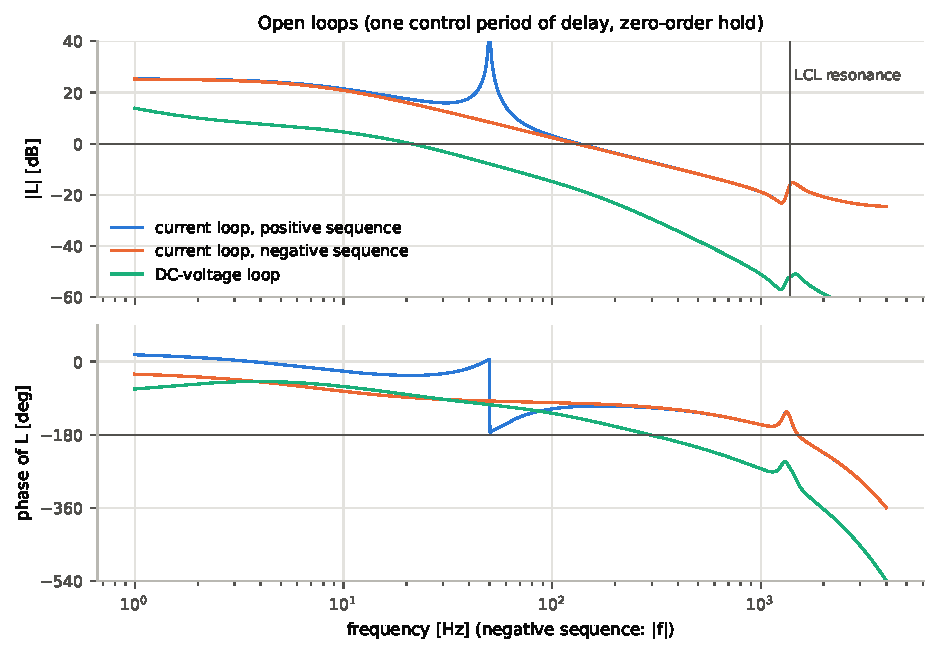
\includegraphics[width=0.92\textwidth]{figures/fig_loops.pdf}
	\caption{Open loops: current loop \eqref{eq:lcur} for the positive and the negative sequence (the positive one has the integrator pole at \SI{50}{\hertz}) and DC-voltage loop \eqref{eq:ludc}. The vertical line marks the LCL resonance.}
	\label{fig:loops}
\end{figure}

\subsection{DC-voltage loop}
\label{sec:udc}

The DC link seen by $u\ped{dc}$ is $C\ped{ser} = \SI{7.2}{\milli\farad}$ with the resistive load. Linearized at the operating point, one pu of active current changes $u\ped{dc}$ (in pu) as
\begin{equation}
	G\ped{u}(s) = \frac{K}{s + a}, \qquad K = \frac{\tfrac32\, \mathrm{Re}(V\ped{conv})\, i\ped{bez}}{C\ped{ser}\, u\ped{dc0}\, u\ped{dc,nom}} = \SI{33.6}{\per\second}, \qquad a = \frac{2}{C\ped{ser}}\Big(\frac{1}{R} + \frac{1}{2R\ped{meas}}\Big) = \SI{55.6}{\radian\per\second},
\end{equation}
where the factor 2 of the pole comes from the load power $u\ped{dc}^2/R$. The loop is
\begin{equation}
	L\ped{u}(z) = \Big(k\ped{p} + k\ped{i}\, t\ped{s} \frac{z}{z-1}\Big)\, T\ped{dd}(z)\, G\ped{u}(z)\, \frac{1}{z},
	\label{eq:ludc}
\end{equation}
with $G\ped{u}(z)$ the zero-order-hold equivalent of $G\ped{u}(s)$ and $T\ped{dd}$ the closed current loop from the $\xi$ reference to the $\xi$ current, obtained from the stationary-frame closed loop $T$ as $T\ped{dd}(f) = \big(T(f + f\ped{0}) + \overline{T(-f + f\ped{0})}\big)/2$. The loop crosses at \SI{21.1}{\hertz} with \ang{97.5} of phase margin: a well-damped and slow loop, about six times slower than the current loop. Its speed matters for the start-up (Section~\ref{sec:startup}) and for load steps: the step from no load to the full load takes the DC link down to about \SI{910}{\volt} in the switched replica (Table~\ref{tab:cases}). Below about \SI{980}{\volt} the converter voltage of the full load, \SI{564}{\volt} phase peak, is beyond the linear range of the modulation, $u\ped{dc}/\sqrt3$ (at \SI{910}{\volt} it would need $|u| = \num{1.07}$): the current PI clips, the bridge rectifies like a diode bridge, and $u\ped{dc}$ recovers from such a dip in \SIrange{0.25}{0.4}{\second}, much slower than the loop.

\subsection{DDSRF-PLL}
\label{sec:pll}

With the positive-sequence feed of Table~\ref{tab:fixes}, the error of the PLL is the $\eta$ component of the decoupled positive sequence after its low-pass filter $F(s) = 1/(\tau s + 1)$, $\tau = 1/\omega$, normalized by the voltage. For small errors the loop is
\begin{equation}
	L\ped{pll}(s) = \frac{\omega(k\ped{p} s + k\ped{i})}{s^2 (\tau s + 1)}, \qquad \tau s^3 + s^2 + \omega k\ped{p}\, s + \omega k\ped{i} = 0,
\end{equation}
the second order loop of the PLL with the filter in it \cite{note_pll3}. The gains of \code{ctrl\_afe\_setup}, $k\ped{p} = 1$, $k\ped{i} = 80$, give a damping of \num{0.99} without the filter but only \ang{33.5} of phase margin with it. Table~\ref{tab:pllgains} compares three sets; the model uses \num{0.32} and \num{8}, the set of \code{frt\_dqpll} after its fix, with the best margin. The lock times of the switched replica (error below \ang{5} from then on) differ less than the margins because the first \SI{12.5}{\milli\second} are spent with the trackers in reset; the start-up current is about the same for the three sets.

\begin{table}[H]
	\centering
	\caption{Gain sets of the DDSRF-PLL: natural frequency and damping without the filter, crossover and phase margin with the filter, lock time in the switched replica.}
	\label{tab:pllgains}
	\rowcolors{2}{tableShade}{white}
	\begin{tabular}{@{} l c c c c c c @{}}
		\toprule
		gain set & $k\ped{p}$ & $k\ped{i}$ & $\omega\ped{n}$ [rad/s] & $\zeta$ & crossover, PM & lock \\
		\midrule
		\code{ctrl\_afe\_setup} & 1 & 80 & 158.5 & 0.99 & \SI{40.7}{\hertz}, \ang{33.5} & \SI{62}{\milli\second} \\
		model (as \code{frt\_dqpll}) & 0.32 & 8 & 50.1 & 1.00 & \SI{15.7}{\hertz}, \ang{58.3} & \SI{44}{\milli\second} \\
		faster & 0.6 & 30 & 97.1 & 0.97 & \SI{27.4}{\hertz}, \ang{45.1} & \SI{38}{\milli\second} \\
		\bottomrule
	\end{tabular}
	\rowcolors{1}{white}{white}
\end{table}

The initial value of the frequency integrator matters more than the gains. From zero, as in \code{frt\_dqpll}, the clamp holds the integrator at \num{0.5} pu, the PLL locks only after \SI{112}{\milli\second}, and in the meantime the current loop works in a frame that turns at half the grid frequency: the start-up current reaches \SI{1228}{\ampere} and the DC link \SI{1513}{\volt} (Figure~\ref{fig:startup}). Started at \num{1} pu, the PLL locks at \SI{44}{\milli\second}.

\subsection{Vienna constraint and neutral point}
\label{sec:vienna}

\paragraph{Window of the zero crossings.} Over one period of the operating point, the pole reference of a phase and its current have opposite signs where the converter voltage, which lags the current by $\delta$, has not yet crossed zero: about $\delta$ after each zero crossing of the current. With the min-max zero sequence \eqref{eq:svm} this window is \ang{8.60} per period, close to $2\delta = \ang{8.68}$ (Figure~\ref{fig:window}). In the window the leg stays at the neutral point \eqref{eq:meff} and the converter voltage of that phase misses a few volts: this distorts the current near its zero crossings (Section~\ref{sec:steady}).

The zero sequence is free in a three-wire system and can be used to give each pole reference the sign of its current: within the limits $|m| \le 1$, choose the zero sequence $v_0$ closest to the min-max one that satisfies $\mathrm{sign}(m\ped{x}) = \mathrm{sign}(i\ped{x})$ for the three phases. At the operating point such a zero sequence exists over 98~\% of the period and the window falls to \ang{2.20} per period. This is not in the model: it needs a change of \code{sv\_pwm\_cm} (C code of the library) or a block after it; the switched replica tests it in Section~\ref{sec:steady}.

\begin{figure}[H]
	\centering
	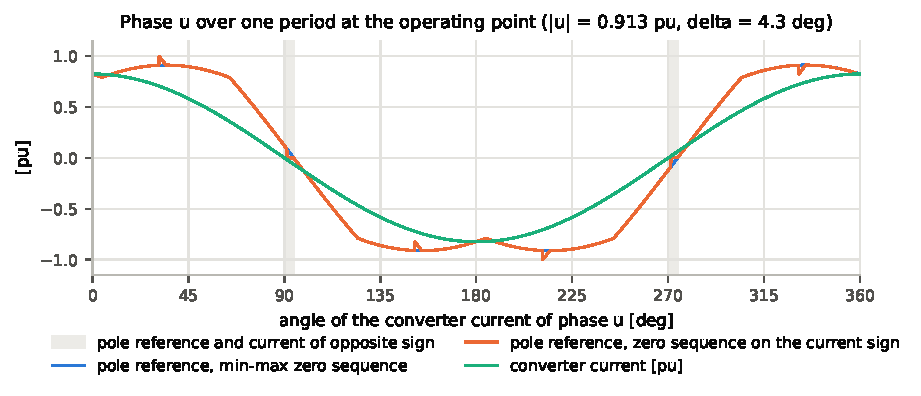
\includegraphics[width=0.92\textwidth]{figures/fig_vienna_window.pdf}
	\caption{Phase u over one period of the operating point: pole reference with the min-max zero sequence, pole reference with the zero sequence that follows the current sign, converter current. The two references differ only near the zero crossings of the three currents; the shaded windows are where the min-max reference and the current have opposite signs.}
	\label{fig:window}
\end{figure}

\paragraph{Neutral point.} A leg is at the neutral point for the fraction $1 - |m\ped{eff}|$ of each carrier period, so the current into the neutral point and the voltage difference of the two halves are
\begin{equation}
	i\ped{np} = \sum_{x = u,v,w} \big(1 - |m\ped{eff,x}|\big)\, i\ped{x}, \qquad \frac{d}{dt}\big(v\ped{C2} - v\ped{C1}\big) = \frac{2\, i\ped{np}}{C\ped{np}}
	\label{eq:np}
\end{equation}
(the measuring dividers are neglected). At the operating point $i\ped{np}$ has no mean value and a third harmonic of \SI{33.0}{\ampere} (peak \SI{43.2}{\ampere}), which gives a ripple of $v\ped{C2} - v\ped{C1}$ of \SI{5.4}{\volt} peak to peak at \SI{150}{\hertz}, \num{0.5}~\% of $u\ped{dc}$. The switched replica gives the same ripple and a mean of \SI{+0.3}{\volt} (Figure~\ref{fig:np}): there is no drift, and no balancing loop is needed in this symmetric case.

% =============================================================
\section{Switched replica: start-up and steady state}
\label{sec:switched}

\subsection{The replica}
\label{sec:replica}

\code{py/vienna\_sim.py} (numpy and numba) integrates the power stage with the step $t\ped{c} = \SI{0.625}{\micro\second}$ of the model (semi-implicit Euler) and runs the control at every peak and valley of the carrier, as the model does:
\begin{itemize}[nosep]
	\item grid emulator with its ramp and second order filter; transformer reduced to its leakage and copper resistance at the secondary, with the no-load voltage $E$ shifted by \ang{30} (no magnetizing branch); LCL filter with the star of the capacitors floating; DC link floating, so the three converter currents add to zero;
	\item Vienna legs by \eqref{eq:pole}: ideal switches and diodes; a phase whose path is blocked for the sign it would take stays at zero current (open phase) while its voltage lies between the two candidate pole voltages; gates by \eqref{eq:gates} with the turn-on delay of the dead time;
	\item control as Section~\ref{sec:control}: 12-bit acquisitions one step late, the first harmonic trackers of the library C code, the DDSRF network and its loop, the DC-voltage PI with back-calculation, the vector PI with clipping, the inverse Park transform and \code{sv\_pwm\_cm} with the sign inversion of the modulator;
	\item options for the comparison, not in the model: the DDSRF-PLL as saved, the initial value of the PLL integrator, no dead time, the zero sequence on the current sign, the lower limit and the anti-windup of the DC-voltage PI, the initial value of the DC-voltage reference, a precharge voltage, a load step, a feed-forward of the capacitor voltage.
\end{itemize}
Not modelled: the clock alignment (one clock), the power meter and the logging, the conduction drops of the devices (diode \SI{2}{\volt}, switch \SI{1.5}{\milli\ohm}) and their RC snubbers. Table~\ref{tab:cases} gives the cases and Table~\ref{tab:startopt} the start-up options; each case runs \SI{1.25}{\second}.

\begin{table}[htbp]
	\centering
	\caption{Switched replica: start-up and steady state. $\hat\imath$: largest converter current and when; $u\ped{dc}$ max and min (min over the first \SI{0.3}{\second}); 2~\%: last time $u\ped{dc}$ is out of \SI{1070}{\volt} $\pm$ 2~\%; lock: PLL error below \ang{5} from then on; THD of the grid and converter currents over the last two periods; $\Delta v\ped{np}$: peak-to-peak ripple of $v\ped{C2} - v\ped{C1}$; window: degrees per period where the pole reference and the current have opposite signs.}
	\label{tab:cases}
	\footnotesize
	\setlength{\tabcolsep}{3.3pt}
	\rowcolors{3}{tableShade}{white}
	\begin{tabular}{@{} l r r r r r r r r r r @{}}
		\toprule
		case & \multicolumn{2}{c}{$\hat\imath$} & \multicolumn{2}{c}{$u\ped{dc}$ [V]} & 2~\% & lock & \multicolumn{2}{c}{THD [\%]} & $\Delta v\ped{np}$ & window \\
		 & [A] & [ms] & max & min & [ms] & [ms] & grid & conv. & [V] & [deg] \\
		\midrule
		as saved: PLL on the negative sequence & 1383 & 119 & 1916 & 784 & 1250 & no & 10.44 & 9.92 & 54.5 & 60.6 \\
		fixed PLL, integrator from 0 & 1228 & 28 & 1513 & 760 & 229 & 112 & 3.42 & 2.80 & 5.4 & 11.0 \\
		\textbf{model as fixed} & \textbf{752} & \textbf{20} & \textbf{1171} & \textbf{758} & \textbf{288} & \textbf{44} & \textbf{3.41} & \textbf{2.79} & \textbf{5.4} & \textbf{11.0} \\
		\quad no dead time & 752 & 20 & 1170 & 760 & 288 & 44 & 3.00 & 2.34 & 5.6 & 10.5 \\
		\quad zero sequence on the current sign & 751 & 20 & 1170 & 758 & 289 & 44 & 2.47 & 1.73 & 6.0 & 2.5 \\
		\quad load connected at \SI{0.2}{\second} & 318 & 219 & 1341 & 913 & 577 & 50 & 3.42 & 2.81 & 5.4 & 11.0 \\
		\quad the same, feed-forward, reference from 1 pu & 318 & 213 & 1125 & 906 & 443 & 50 & 3.44 & 2.93 & 5.4 & 9.5 \\
		\bottomrule
	\end{tabular}
	\rowcolors{1}{white}{white}
\end{table}

\subsection{Start-up}
\label{sec:startup}

\begin{figure}[tb]
	\centering
	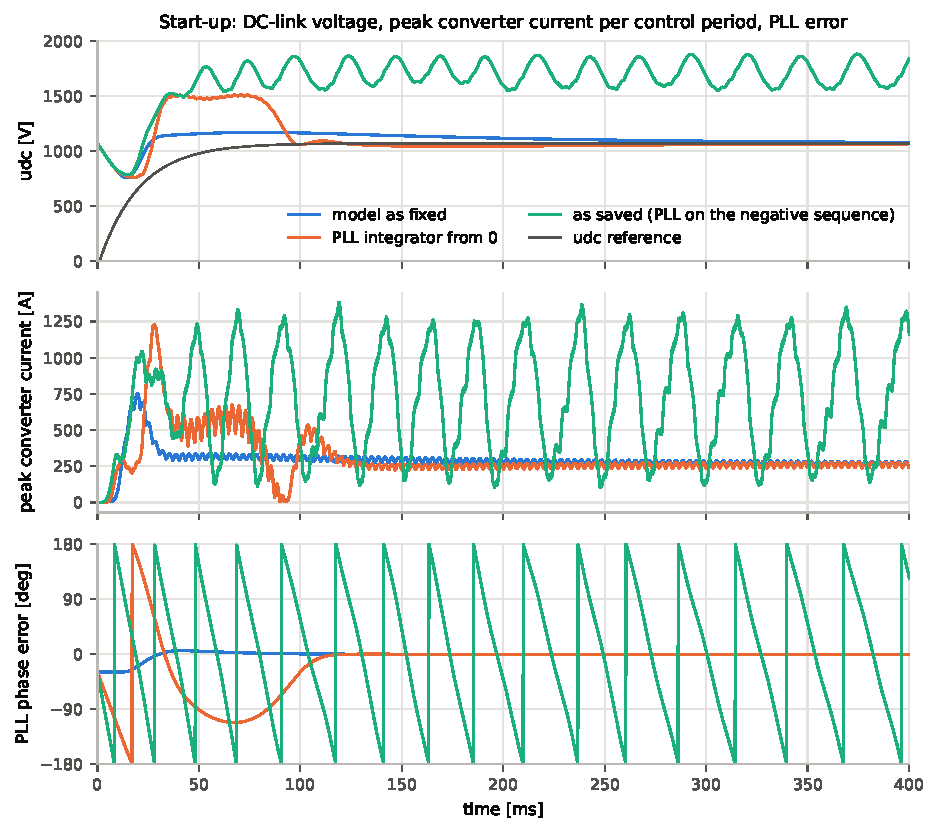
\includegraphics[width=0.85\textwidth]{figures/fig_startup.pdf}
	\caption{Start-up in the switched replica: DC-link voltage with the reference of the model, largest converter current per control period, phase error of the PLL. Model as fixed, fixed PLL with the integrator started from 0, PLL as saved.}
	\label{fig:startup}
\end{figure}

Figure~\ref{fig:startup} compares the model as saved (PLL on the negative sequence), the fixed PLL started from zero and the model as fixed. As saved, the phase error of the PLL never stops turning, the current loop works in a wrong frame and the DC link oscillates between \SI{1.6}{} and \SI{1.9}{\kilo\volt}. With the fixed PLL started at \num{1} pu the model starts in about \SI{0.3}{\second}, but with a current peak of \SI{752}{\ampere} (\num{2.3} pu) at \SI{20}{\milli\second}. Figure~\ref{fig:startuppi} shows how it builds up:
\begin{itemize}[nosep]
	\item for the first \SI{15}{\milli\second} the grid voltage is still small and the load drains the DC link with $R C\ped{ser} = \SI{36}{\milli\second}$: $u\ped{dc}$ falls to \SI{758}{\volt}, below the level of the diodes, $\sqrt3 E = \SI{986}{\volt}$;
	\item the DC-voltage reference rises from zero (step at \SI{1}{\milli\second} and \SI{20}{\milli\second} filter) and stays below $u\ped{dc}$ for the whole start, so the error $e$ of the DC-voltage PI is negative. The PI is in velocity form with back-calculation: it stores $x = i\ped{\xi}^* - k\ped{p} e$ also while its output is clamped, so each step adds $k\ped{p} \Delta e + k\ped{i} t\ped{s} e$ to the last, clamped output. The error starts at \num{-1} pu, the output at its lower limit, \num{-1.65} pu, and the stored state is $-1.65 + 4 = \num{+2.35}$ pu. As the reference rises and $u\ped{dc}$ falls, the error shrinks and the output rises with it: it turns positive at \SI{8}{\milli\second} and reaches \num{1.16} pu at \SI{15}{\milli\second}, with $u\ped{dc}$ still \SI{220}{\volt} above its reference. The PI asks for an active current that the DC voltage does not need;
	\item the current PI has no feed-forward of the grid voltage: its integrators must build the whole converter voltage while the grid voltage rises, and the current overshoots its reference, \num{2.26} pu (\SI{743}{\ampere}) at \SI{20}{\milli\second} against \num{1.14} pu. This is the peak;
	\item the current then recharges the DC link above its reference, to \SI{1171}{\volt} (+9.4~\%), and the bridge cannot give the energy back: only the load brings $u\ped{dc}$ down, within 2~\% after \SI{288}{\milli\second}.
\end{itemize}
Item 7 of the design check prints the threshold of the second point: the output of the PI turns positive when the error rises above $-x/(k\ped{p} + k\ped{i} t\ped{s}) = \num{-0.59}$ pu (\num{-0.52} pu in the replica, where the integral of the first steps adds to the threshold).

\begin{figure}[tb]
	\centering
	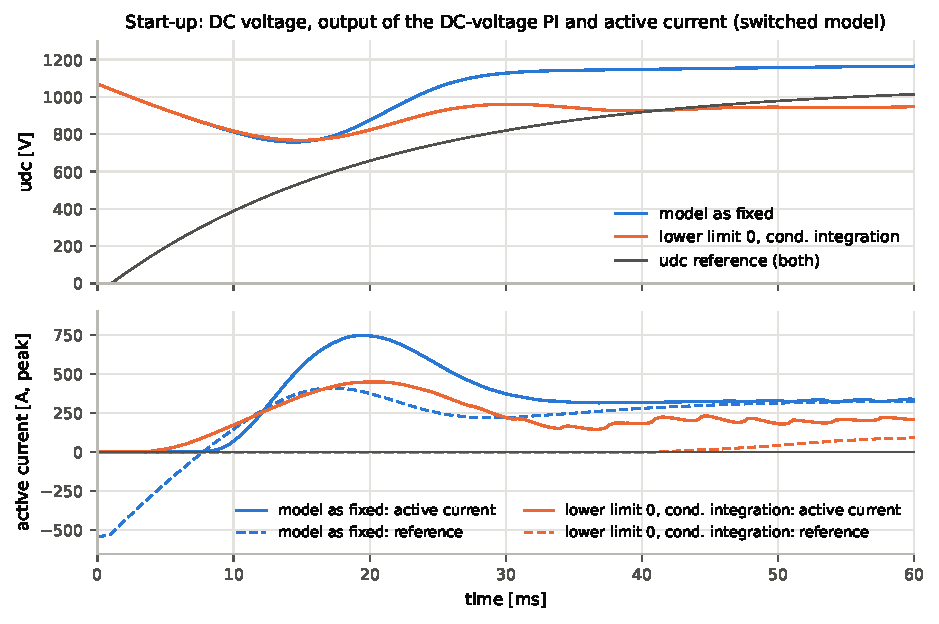
\includegraphics[width=0.85\textwidth]{figures/fig_startup_pi.pdf}
	\caption{First \SI{60}{\milli\second} of the start-up in the switched replica, model as fixed and DC-voltage PI with lower limit 0 and conditional integration: DC-link voltage and its reference (top); active current and its reference, the output of the DC-voltage PI (bottom).}
	\label{fig:startuppi}
\end{figure}

Table~\ref{tab:startopt} and Figure~\ref{fig:startupopt} give the options. Each of the two working changes removes one of the two causes; each half of a change alone is not enough.
\begin{itemize}
	\item \textbf{DC-voltage PI with lower limit 0 and conditional integration.} The bridge cannot give a negative active current, so 0 is the right lower limit; with conditional integration the integrator holds while the output is clamped, in place of the back-calculation. The reference of the current stays at zero until \SI{41}{\milli\second}, when $u\ped{dc}$ has fallen below the rising reference (Figure~\ref{fig:startuppi}). The peak falls to \SI{456}{\ampere} and $u\ped{dc}$ does not overshoot. These \SI{456}{\ampere} are the current that the rising grid voltage drives through the filter while the current loop, still without feed-forward, holds its zero reference only with a large error. With the lower limit at 0 and the back-calculation kept, the output starts its rise from 0 instead of \num{-1.65} pu and the peak is \SI{1068}{\ampere}; with conditional integration and the limit kept at \num{-1.65} pu, the reference of the current stays negative until \SI{50}{\milli\second}, which the bridge cannot follow: the DC link falls to \SI{647}{\volt} and the diodes recharge it at full grid voltage (\SI{587}{\ampere}).
	\item \textbf{Feed-forward of the capacitor voltage and DC-voltage reference from the measured voltage.} The feed-forward $u\ped{ff} = -(\sqrt3\, u\ped{bez}/u\ped{dc})\, v\ped{c}$ on the output of the current PI, in the $\xi\eta$ frame with the sample advanced by $1.5\, t\ped{s}$, lets the current follow its reference. With the reference of $u\ped{dc}$ started from the measured voltage (here \num{1} pu), the DC-voltage PI asks for current only to recharge the DC link, up to its limit of \num{1.65} pu (\SI{542}{\ampere}): the peak is \SI{455}{\ampere} and $u\ped{dc}$ does not overshoot. The steady state is the same (THD \num{3.43}~\%): with this filter the feed-forward does not upset the damping of the LCL mode. The reference from \num{1} pu without the feed-forward gives \SI{782}{\ampere}, the feed-forward with the reference from zero \SI{511}{\ampere} and an overshoot to \SI{1185}{\volt}.
\end{itemize}
The two changes together give the same as the second one alone. The feed-forward with the reference from zero should not be combined with the changed PI: the current then stays near zero during the ramp of the grid voltage, the load drains the DC link to \SI{611}{\volt}, and the recharge at full grid voltage reaches \SI{677}{\ampere}.

With either change $u\ped{dc}$ comes back to its reference slowly, within 2~\% after \SI{317}{\milli\second} and \SI{235}{\milli\second}: below about \SI{980}{\volt} the current PI clips (Section~\ref{sec:udc}) and the bridge rectifies like a diode bridge. The dip to about \SI{770}{\volt} is the load draining the DC link while the grid voltage rises from zero, a condition of the test rather than of the converter; a precharge to \SI{980}{\volt} changes little. Connecting the load later does not help either (Table~\ref{tab:cases}): without the feed-forward the start-up current alone charges the unloaded DC link to \SI{1341}{\volt}; with it and the reference from \num{1} pu the start draws less than \SI{30}{\ampere}, but the DC link still creeps up to \SI{1125}{\volt} in \SI{0.2}{\second}. Near zero load the current cannot be held at zero: the short current pulses that remain are rectified into the DC link (about \SI{1.8}{\kilo\watt} here) and nothing takes the energy back, so a Vienna rectifier needs a minimum load to hold its DC voltage.

\begin{table}[htbp]
	\centering
	\caption{Start-up options in the switched replica, each a change of the model as fixed. Columns as in Table~\ref{tab:cases}; $u\ped{dc}$ max \SI{1070}{\volt} is the precharge: no overshoot.}
	\label{tab:startopt}
	\footnotesize
	\rowcolors{3}{tableShade}{white}
	\begin{tabular}{@{} l r r r r r r @{}}
		\toprule
		change & \multicolumn{2}{c}{$\hat\imath$} & \multicolumn{2}{c}{$u\ped{dc}$ [V]} & 2~\% & THD grid \\
		 & [A] & [ms] & max & min & [ms] & [\%] \\
		\midrule
		none (model as fixed) & 752 & 20 & 1171 & 758 & 288 & 3.41 \\
		\textbf{DC-voltage PI: lower limit 0, conditional integration} & \textbf{456} & \textbf{19} & \textbf{1070} & \textbf{767} & \textbf{317} & \textbf{3.39} \\
		\quad lower limit 0 only (back-calculation kept) & 1068 & 17 & 1251 & 763 & 338 & 3.41 \\
		\quad conditional integration only (limit $-1.65$ pu kept) & 587 & 26 & 1070 & 647 & 346 & 3.42 \\
		DC-voltage reference from 1 pu & 782 & 16 & 1084 & 785 & 263 & 3.42 \\
		feed-forward, reference from 0 & 511 & 23 & 1185 & 704 & 307 & 3.42 \\
		\textbf{feed-forward, reference from 1 pu} & \textbf{455} & \textbf{17} & \textbf{1070} & \textbf{772} & \textbf{235} & \textbf{3.43} \\
		feed-forward and the changed PI, reference from 0 & 677 & 27 & 1070 & 611 & 306 & 3.44 \\
		DC link precharged to \SI{980}{\volt} & 724 & 20 & 1136 & 701 & 249 & 3.40 \\
		\bottomrule
	\end{tabular}
	\rowcolors{1}{white}{white}
\end{table}

\begin{figure}[htbp]
	\centering
	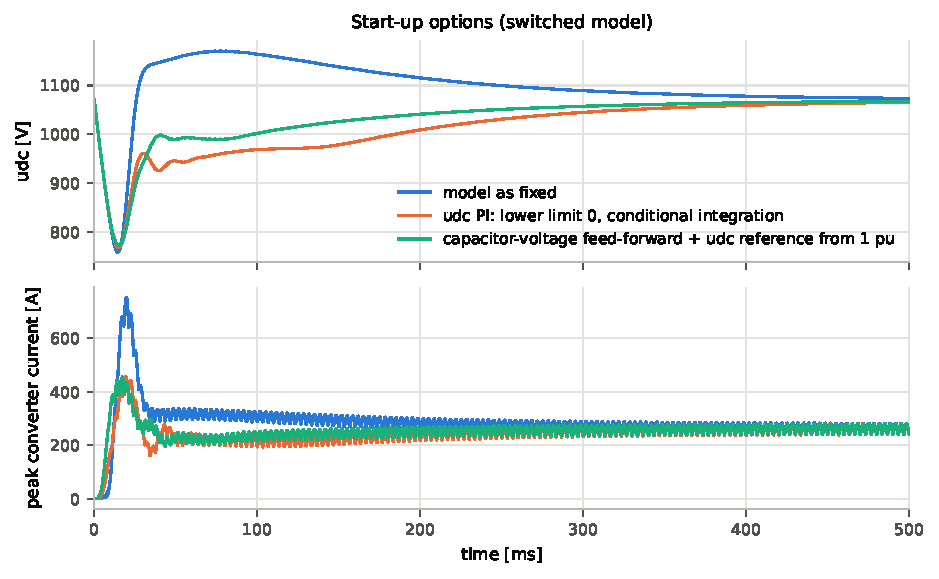
\includegraphics[width=0.85\textwidth]{figures/fig_startup_options.pdf}
	\caption{Start-up options in the switched replica: model as fixed, DC-voltage PI with lower limit 0 and conditional integration, feed-forward of the capacitor voltage with the DC-voltage reference started from the measured voltage.}
	\label{fig:startupopt}
\end{figure}

\subsection{Steady state}
\label{sec:steady}

In steady state (Figure~\ref{fig:steady}) the grid current has a fundamental of \SI{275.1}{\ampere} peak and a THD of \num{3.41}~\%, with \num{2.0}~\% of 5th, \num{1.6}~\% of 7th, \num{1.1}~\% of 11th and \num{0.9}~\% of 13th harmonic (Figure~\ref{fig:spectrum}); the reactive current is zero. The low-order harmonics come mostly from the zero crossings: the converter current minus its fundamental shows a step at each zero crossing of the current, where the leg stays at the neutral point and a phase is open for a short time (one phase open \num{1.24}~\% of the time). The window of the replica is \ang{11.0} per period, a little more than the \ang{8.6} of the linear estimate, because the switching ripple makes the current change sign several times near its zero crossings. The dead time adds \num{0.4}~\% of THD.

The zero sequence on the current sign (Section~\ref{sec:vienna}), computed with the sign of the reference current $1.5\, t\ped{s}$ ahead, reduces the window to \ang{2.5} per period and the THD to \num{2.47}~\% (5th \num{1.2}~\%, 7th \num{0.9}~\%), with the same start-up and a neutral-point ripple of \SI{6.0}{\volt} instead of \SI{5.4}{\volt}.

\begin{figure}[H]
	\centering
	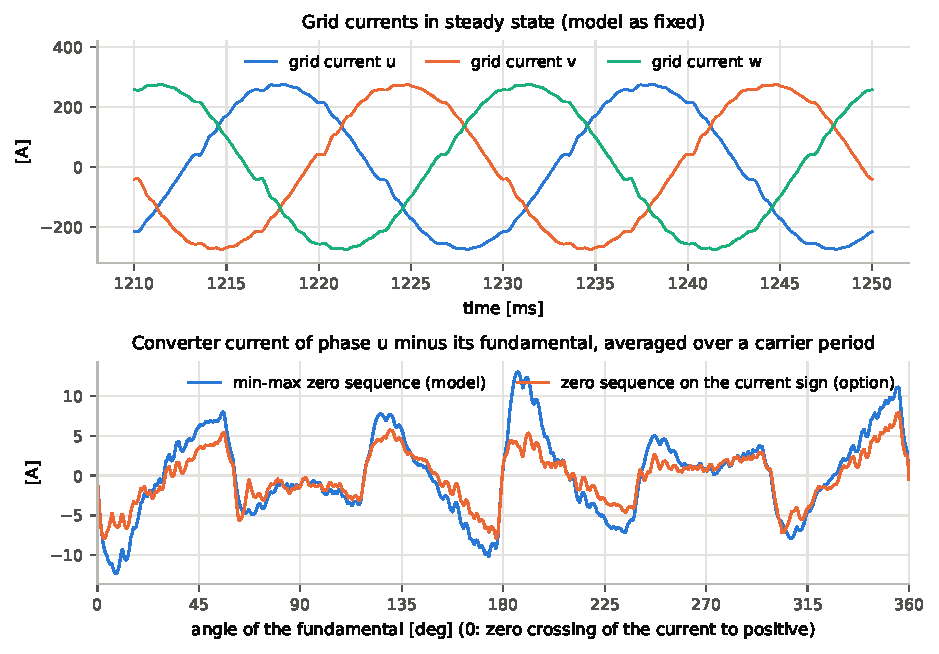
\includegraphics[width=0.92\textwidth]{figures/fig_steady.pdf}
	\caption{Steady state in the switched replica. Top: grid currents. Bottom: converter current of phase u minus its fundamental, averaged over a carrier period, over one period from its positive-going zero crossing, with the min-max zero sequence of the model and with the zero sequence on the current sign.}
	\label{fig:steady}
\end{figure}

\begin{figure}[H]
	\centering
	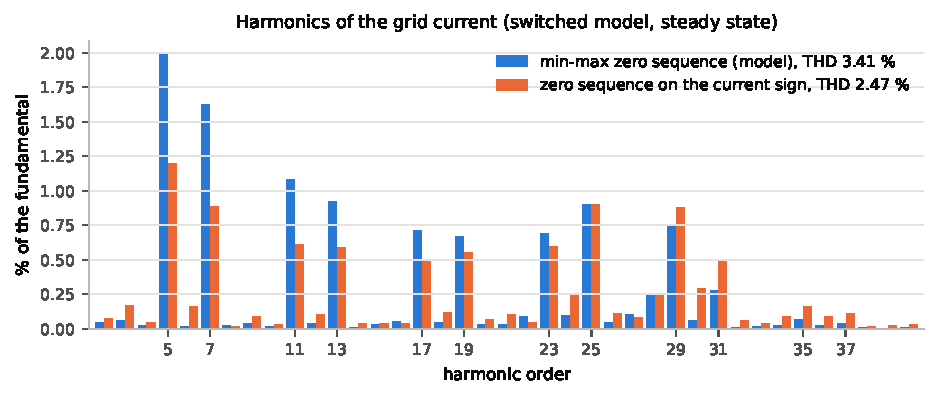
\includegraphics[width=0.92\textwidth]{figures/fig_spectrum.pdf}
	\caption{Harmonics of the grid current in steady state (switched replica, two periods), in \% of the fundamental.}
	\label{fig:spectrum}
\end{figure}

\begin{figure}[H]
	\centering
	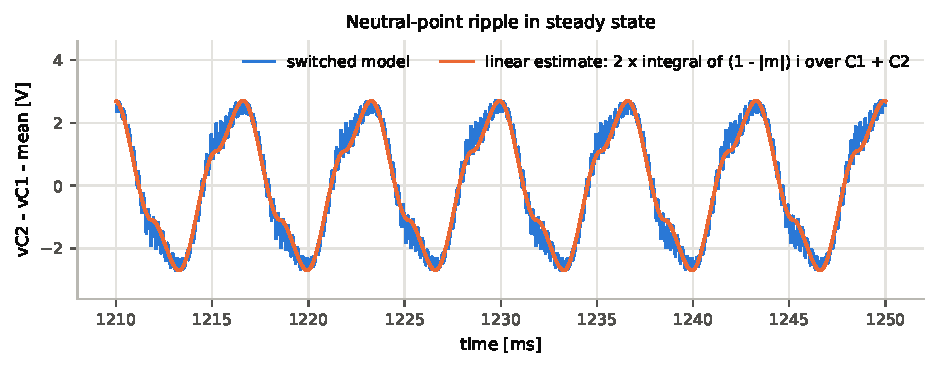
\includegraphics[width=0.92\textwidth]{figures/fig_neutral_point.pdf}
	\caption{Ripple of $v\ped{C2} - v\ped{C1}$ in steady state: switched replica and linear estimate \eqref{eq:np}.}
	\label{fig:np}
\end{figure}

% =============================================================
\section{Open points and recommendations}
\label{sec:open}

\begin{enumerate}
	\item \textbf{Run the revised model in MATLAB.} The model was opened in MATLAB and its scoped tag fixed (Table~\ref{tab:fixes}), but no run has been compared with the replica yet. The initialization prints the design check and the result of the two model checks; the start-up and the steady state of the model should match Table~\ref{tab:cases} (model as fixed).
	\item \textbf{Start-up current} (Section~\ref{sec:startup}). Recommended, one of two changes, each about \SI{455}{\ampere} instead of \SI{752}{\ampere} in the replica and no overshoot:
	\begin{enumerate}[label=(\alph*), nosep]
		\item in \code{udc\_ctrl}, the lower limit of the Saturation at 0 and conditional integration: the Unit Delay of the PI keeps its state while the output is clamped, in place of $i\ped{\xi}^* - k\ped{p} e$. A change of one subsystem of the model, with the reference of the model unchanged;
		\item a feed-forward of the measured capacitor voltage on the output of the current PI (sample advanced by $1.5\, t\ped{s}$, scaled by $\sqrt3\, u\ped{bez}/u\ped{dc}$) and a DC-voltage reference that starts from the measured $u\ped{dc}$ (the low-pass block of the library has no initial state, so the filter must be initialized or replaced). The feed-forward also helps the current loop in grid transients.
	\end{enumerate}
	Both together give the same as (b); do not combine (a) with the feed-forward while the reference still starts from zero (Table~\ref{tab:startopt}). Enabling the PWM only after the lock of the PLL is a further option. The rectifier also needs a minimum load: with no load the DC link creeps up.
	\item \textbf{Voltage margin} (Section~\ref{sec:udc}). At \SI{1070}{\volt} the converter voltage of the full load needs \num{0.913} of the linear range of the modulation; below about \SI{980}{\volt} it is out of range. After the start and after a step to the full load (dip to about \SI{910}{\volt}) the current PI clips, the bridge rectifies like a diode bridge and $u\ped{dc}$ recovers in \SIrange{0.25}{0.4}{\second}. A faster recovery needs a higher DC-voltage reference, if the devices allow it, or smaller load steps.
	\item \textbf{Distortion at the zero crossings} (Sections~\ref{sec:vienna} and \ref{sec:steady}). A zero sequence that follows the sign of the current lowers the THD of the grid current from \num{3.4}~\% to \num{2.5}~\%. It needs a change of \code{sv\_pwm\_cm} (C code of the library, used by other models) or a block between it and the modulator.
	\item \textbf{LCL resonance} (Section~\ref{sec:lcl}). At \SI{1381}{\hertz}, just above $f\ped{s}/6$, the mode keeps its passive damping (5.8~\%). With a stiffer grid it moves up and the converter-current loop cannot damp it; if the filter or the transformer changes, check it again, or add active damping (capacitor current) or move the loop to the grid current.
	\item \textbf{Neutral point.} There is no balancing loop: the zero-sequence PI is made for modules in parallel and its output gain is 0. In this symmetric case the mean unbalance is \SI{0.3}{\volt}; with unbalanced grids, unequal capacitors or unequal devices a loop on the zero sequence will be needed. The zero sequence on the current sign uses the same degree of freedom: the two must be designed together.
	\item \textbf{Fault ride-through.} The data of test 25.4 of VDE-AR-N 4110 are computed but not applied, and the Vienna control has no FRT logic; the DDSRF-PLL is ready for asymmetric dips \cite{note_pll3}, the rest of the control is not.
	\item \textbf{Housekeeping.} Ten Goto blocks have no reader; \code{init\_model\_legacy.m} can be deleted once the new initialization is adopted.
\end{enumerate}

% =============================================================
\section{Files and how to reproduce}
\label{sec:files}

\begin{itemize}
	\item The model folder \code{vienna\us rectifier}, in \code{foundations\us of\us power\us electronics} of \cite{model_repo}:
	\begin{itemize}[nosep]
		\item \code{vienna\_rectifier.slx}, the model;
		\item \code{init\_model.m}, the initialization: run it from this folder, then run the model;
		\item \code{vienna\_rectifier\_private.m} and the functions of \code{private/}: the parameter functions, the design check \code{vienna\_design}, the bus of the power meter, the path of the library and the two model checks;
		\item \code{init\_model\_legacy.m}, the old initialization, and the README with the list of the legacy names.
	\end{itemize}
	\item This folder:
	\begin{itemize}[nosep]
		\item \code{py/vienna\_sim.py}: the switched replica, \code{run(\ldots)} with the options of Section~\ref{sec:replica};
		\item \code{py/vienna\_design\_check.py}: the linear checks of \code{vienna\_design} and the cases of Tables~\ref{tab:cases} and \ref{tab:startopt}. Run \code{python3 vienna\_design\_check.py ../figures} from \code{py/} (a few seconds with numba): it writes every figure of this note and the numbers to \code{figures/\allowbreak vienna\us design\us check\us output.txt}.
	\end{itemize}
	\item The library \cite{library_repo}: the Vienna bridge \code{vienna\us rectifier\us ideal\us switch\us based\us model}, the three-level PWM, the C callers \code{sv\_pwm\_cm} and \code{first\us harmonic\us tracker}, the classes \code{ctrl\_afe\_setup}, \code{hw\us afe\us three\us phase\us setup} and \code{grid\us three\us phase\us emulator}.
\end{itemize}

% =============================================================
\begin{thebibliography}{9}
	\raggedright
	\bibitem{model_repo} pwr-control, \emph{modelization-and-control}, repository, folder \code{foundations\us of\us power\us electronics/\allowbreak vienna\us rectifier} (model \code{vienna\_rectifier.slx}, README with the design check of November 2026). \url{https://github.com/pwr-control/modelization-and-control}
	\bibitem{library_repo} pwr-control, \emph{library}, repository: semiconductor bridges, modulators, C callers (\code{sv\_pwm\_cm}, \code{first\_harmonic\_tracker}), setup classes. \url{https://github.com/pwr-control/library}
	\bibitem{note_pll3} D. Bagnara, \emph{Three-phase grid PLLs under grid faults: dq-PLL, DDSRF-PLL and FHT-PLL of the model frt\_dqpll}, pwr-control technical note, rev.~00, November 2026, \code{repos\_doc/\allowbreak three\us phase\us plls\us comparison} of \emph{repositories-documentation}.
	\bibitem{kolar1997} J. W. Kolar and F. C. Zach, ``A novel three-phase utility interface minimizing line current harmonics of high-power telecommunications rectifier modules,'' \emph{IEEE Transactions on Industrial Electronics}, vol.~44, no.~4, pp.~456--467, 1997.
	\bibitem{kolar2013} J. W. Kolar and T. Friedli, ``The essence of three-phase PFC rectifier systems---Part I,'' \emph{IEEE Transactions on Power Electronics}, vol.~28, no.~1, pp.~176--198, 2013.
	\bibitem{dannehl2009} J. Dannehl, C. Wessels and F. W. Fuchs, ``Limitations of voltage-oriented PI current control of grid-connected PWM rectifiers with LCL filters,'' \emph{IEEE Transactions on Industrial Electronics}, vol.~56, no.~2, pp.~380--388, 2009.
	\bibitem{parker2014} S. G. Parker, B. P. McGrath and D. G. Holmes, ``Regions of active damping control for LCL filters,'' \emph{IEEE Transactions on Industry Applications}, vol.~50, no.~1, pp.~424--432, 2014.
	\bibitem{rodriguez2007} P. Rodr\'iguez, J. Pou, J. Bergas, J. I. Candela, R. P. Burgos and D. Boroyevich, ``Decoupled double synchronous reference frame PLL for power converters control,'' \emph{IEEE Transactions on Power Electronics}, vol.~22, no.~2, pp.~584--592, 2007.
\end{thebibliography}

\end{onehalfspace}
\end{document}
